%-----------------------------------------------------------------------------
%
%          PHYSICS  M.S.     THESIS
%          JUSTIN A. VASEL
%
%          This began as the template offered by the University of Minnesota, 
%          but I've made a few changes here and there...  
%
%          -->  thesis.tex
%
%-----------------------------------------------------------------------------



%-------------------------------------------------------------------------------
%    //  P R E A M B L E
%===============================================================================
	\documentclass[12pt, twoside, fleqn]{./Styles/mnthesis}
	
	%%%%%%%%%%%%%%%%%%%%%%%%%
	%   //  PACKAGES        %
	%%%%%%%%%%%%%%%%%%%%%%%%%
		% // EPS Files
			\usepackage{epsfig}
			\usepackage{epic}
			\usepackage{eepic}

		% // Graphics and Figures
			\usepackage{graphicx}
			\usepackage{float}
			\usepackage[font=small]{caption}
			\usepackage{subcaption}
			\usepackage{wrapfig}

		% // TikZ
			\usepackage[usenames,dvipsnames]{xcolor}
			\usepackage{tikz}
				\usetikzlibrary{decorations.pathmorphing,decorations.markings,trees,arrows}
				\pgfdeclarelayer{background}
				\pgfdeclarelayer{foreground}
				\pgfsetlayers{background,main,foreground}
			\usepackage{pgfplots}

		% // Tables
			\usepackage{array}
			\usepackage{multirow}
			\usepackage{longtable}
			\usepackage{booktabs}

		% // Maths
			\usepackage{amsmath}
			\usepackage{amssymb}
			\usepackage{mathrsfs}

		% // HEP
			\usepackage{braket}			% Dirac notation
			\usepackage{hepparticles}	% Format particle processes
			\usepackage{hepnames}		% Format particle names

		% // Hyperlinks
			\usepackage[colorlinks=true, urlcolor=BrickRed, linkcolor=Black, citecolor=Black]{hyperref}		% href
			\usepackage{url}			% Don't use, makes text unicode

		% // Misc.
			\usepackage[emulate=hepunits,sepfour=true,digitsep=comma]{siunitx}		% Handles unit formatting
				\DeclareSIUnit\year{yr}
			\usepackage{lipsum}			% Generate Lorem Ipsum text
			\usepackage{setspace}
			\usepackage{titlesec}
			\usepackage[leftmargin=2in,rightmargin=0in,vskip=0.5in]{./Styles/quoting}
			\usepackage{lettrine}
			\usepackage{lineno}
			\usepackage{listings}

		% // Unknown
			\usepackage{./Styles/bigstrut}		% No idea what this does


	%%%%%%%%%%%%%%%%%%%%%%
	%   //  FONTS        %
	%%%%%%%%%%%%%%%%%%%%%%

		% // fontenc may be redundant. fontspec needed to use system fonts
		\usepackage{fontspec}
		\usepackage{anyfontsize}
		\usepackage[utf8x]{inputenc}

		\setmainfont[Ligatures=TeX]{Adobe Caslon}

		% // DEFINE \neue as `Helvetica Neue'
		% // DEFINE \light as `Helvetica Neue UltraLight'
		% // DEFINE \minion as `Minion Pro'

		\newfontfamily\garamond[]{Medio}
		\newfontfamily\neue[]{Helvetica Neue}
		\newfontfamily\light[]{Helvetica Neue UltraLight}
		\newfontfamily\minion[]{Minion Pro}
		\newfontfamily\caslon[]{Adobe Caslon Pro}
		\newfontfamily\bask[]{Baskerville}

		% // Custom formatting for chapter titles
		\titleformat{\chapter}[display]{\nolinenumbers \raggedright \linespread{0.5} \huge}{\chaptertitlename\ \vspace{0.25in} \thechapter}{0pt}{\fontsize{40}{50}\selectfont}
		
		% // Custom formatting for captions
		\DeclareCaptionLabelFormat{smallcaps}{\normalsize \minion \textsc{#1 #2}}
		\captionsetup[figure]{name=Fig.}
		\captionsetup{labelformat=smallcaps, labelfont=bf, labelsep=period}



	%%%%%%%%%%%%%%%%%%%%%%
	%   //  GRAPHICS     %
	%%%%%%%%%%%%%%%%%%%%%%
		
		% // Set path to look for images and graphics extension types
		\graphicspath{ {../images/}{../images/Intro/}{../images/Neutrinos/}{../images/Supernovae/}{../images/Snews/}{../images/Halo/}{../images/Conclusion/} }
		\DeclareGraphicsExtensions{.eps,.pdf,.png}
		
		
		
	%%%%%%%%%%%%%%%%%%%%%%
	%   //  OTHER        %
	%%%%%%%%%%%%%%%%%%%%%%

		% // Pull in custom definitions
		%-----------------------------------------------------------------------------
%
%          PHYSICS  M.S.     THESIS
%          JUSTIN A. VASEL
%
%          This began as the template offered by the University of Minnesota, 
%          but I've made a few changes here and there...  
%
%          -->  my_definitions.tex
%
%-----------------------------------------------------------------------------

%% MATHS
\newcommand{\COS}{{\mathrm{cos}}}
\newcommand{\SIN}{{\mathrm{sin}}}

% energy (prefix: e)
\newcommand{\eGeV}[1]{\SI{#1}{\GeV}}
\newcommand{\eMeV}[1]{\SI{#1}{\MeV}}
\newcommand{\ekeV}[1]{\SI{#1}{\keV}}
\newcommand{\eeV}[1]{\SI{#1}{\eV}}

% mass (prefix: m)
\newcommand{\mGeV}[1]{\SI[per=slash,eVcorrb=0.4ex]{#1}{\giga\eVperc\squared}}
\newcommand{\mMeV}[1]{\SI[per=slash,eVcorrb=0.4ex]{#1}{\mega\eVperc\squared}}
\newcommand{\mkeV}[1]{\SI[per=slash,eVcorrb=0.4ex]{#1}{\kilo\eVperc\squared}}
\newcommand{\mmeV}[1]{\SI[per=slash,eVcorrb=0.4ex]{#1}{\eVperc\squared}}


%% HEADINGS
\newcommand{\CONT}{\noindent}
\newcommand{\FIG}{Fig. \nolinebreak }
\newcommand{\FIGS}{Figs. \nolinebreak }
\newcommand{\SEC}{Sec.\ }
\newcommand{\SECS}{Secs.\ }
\newcommand{\TAB}{Table }
\newcommand{\TABS}{Tables }
\newcommand{\EQ}{Eq.\nolinebreak \ }
\newcommand{\EQS}{Eqs.\nolinebreak \ }
\newcommand{\APP}{Appendix }
\newcommand{\APPS}{Appendices }
\newcommand{\CHP}{Chapter }
\newcommand{\CHPS}{Chapters }


%% OTHER
\def\imagetop#1{\vtop{\null\hbox{#1}}}

\newcommand{\plan}[1] {
	\noindent {\color{BrickRed} [#1]} \\
}

\newcommand{\filler} {
	{\color{MidnightBlue} \lipsum}
}

\newcommand{\scaps}[1] {
	\minion \textsc{#1}\normalfont
}

\newcommand{\chapterIntro}[2] {
	\noindent
	\lettrine[lines=4,nindent=4pt]{#1}{\scaps{#2}}
}

\definecolor{light-gray}{gray}{0.3}

\newcommand{\he}{
	$^3$He
}

\newcommand{\confirm}[1]{
	{\color{Rhodamine} #1}
}

% place an inline node that is remembered for tikz
% \tikzremember{<node name>}
%   note: you have to compile twice
\newcommand{\tikzremember}[1]{{
  \tikz[remember picture,overlay]{\node (#1) at (0,11pt) { };}
}}

\colorlet{punct}{red!60!black}
\definecolor{background}{HTML}{EEEEEE}
\definecolor{delim}{RGB}{20,105,176}
\colorlet{numb}{magenta!60!black}

\lstdefinelanguage{json}{
    basicstyle=\footnotesize\ttfamily,
    stepnumber=1,
    numbersep=8pt,
    showstringspaces=false,
    extendedchars=\true,
    frame=lines,
    backgroundcolor=\color{background},
    literate=
     *{0}{{{\color{numb}0}}}{1}
      {1}{{{\color{numb}1}}}{1}
      {2}{{{\color{numb}2}}}{1}
      {3}{{{\color{numb}3}}}{1}
      {4}{{{\color{numb}4}}}{1}
      {5}{{{\color{numb}5}}}{1}
      {6}{{{\color{numb}6}}}{1}
      {7}{{{\color{numb}7}}}{1}
      {8}{{{\color{numb}8}}}{1}
      {9}{{{\color{numb}9}}}{1}
      {:}{{{\color{punct}{:}}}}{1}
      {,}{{{\color{punct}{,}}}}{1}
      {\{}{{{\color{delim}{\{}}}}{1}
      {\}}{{{\color{delim}{\}}}}}{1}
      {[}{{{\color{delim}{[}}}}{1}
      {]}{{{\color{delim}{]}}}}{1},
}

\lstdefinelanguage{object-c}{
    basicstyle=\footnotesize\ttfamily,
    stepnumber=1,
    numbersep=8pt,
    showstringspaces=false,
    extendedchars=\true,
    frame=lines,
    backgroundcolor=\color{background},
    literate=
     *{0}{{{\color{numb}0}}}{1}
      {1}{{{\color{numb}1}}}{1}
      {2}{{{\color{numb}2}}}{1}
      {3}{{{\color{numb}3}}}{1}
      {4}{{{\color{numb}4}}}{1}
      {5}{{{\color{numb}5}}}{1}
      {6}{{{\color{numb}6}}}{1}
      {7}{{{\color{numb}7}}}{1}
      {8}{{{\color{numb}8}}}{1}
      {9}{{{\color{numb}9}}}{1}
      {:}{{{\color{punct}{:}}}}{1}
      {,}{{{\color{punct}{,}}}}{1}
      {=}{{{\color{punct}{=}}}}{1}
      {"}{{{\color{punct}{"}}}}{1}
      {@}{{{\color{punct}{@}}}}{1}
      {\{}{{{\color{delim}{\{}}}}{1}
      {\}}{{{\color{delim}{\}}}}}{1}
      {[}{{{\color{delim}{[}}}}{1}
      {]}{{{\color{delim}{]}}}}{1}
      {)}{{{\color{delim}{)}}}}{1}
      {(}{{{\color{delim}{(}}}}{1},
}


%-----------------------------------------------------------------------------
%-----------------------------------------------------------------------------
		%-----------------------------------------------------------------------------
%
%          PHYSICS  M.S. THESIS
%          JUSTIN A. VASEL
%
%          -->  TeX/Definitions/tikz_definitions.tex
%
%          This began as the template offered by the University of Minnesota, 
%          but I've made a few changes here and there...  
%
%-----------------------------------------------------------------------------

 % place an inline node that is remembered for tikz
    % \tikzremember{<node name>}
    %   note: you have to compile twice
    \newcommand{\tikzremember}[1]{{
      \tikz[remember picture,overlay]{\node (#1) at (0,11pt) { };}
    }}

    % Used in the supernova classification TikZ diagram
    \definecolor{light-gray}{gray}{0.3}


% // Decoration for Feynman diagram symbols
  \tikzset{
      photon/.style={
        decorate, 
        decoration={snake}, 
        draw=red
    },
      fermion-in/.style={
          draw=black, 
      postaction={decorate},
          decoration={
              markings,
        mark=at position .55 with {\arrow[draw=black]{<}}
      }
    },
    fermion-out/.style={
          draw=black, 
      postaction={decorate},
          decoration={
              markings,
        mark=at position .55 with {\arrow[draw=black]{>}}
      }
    },
      gluon/.style={
          decorate, 
      draw=magenta,
          decoration={
              coil,
        amplitude=4pt, 
        segment length=5pt
      }
    } 
  }

% // Decoration for Data Flow diagram
% // Defines a `datastore' shape for use in DFDs.  This inherits from a
% rectangle and only draws two horizontal lines.
\makeatletter
\pgfdeclareshape{datastore}{
  \inheritsavedanchors[from=rectangle]
  \inheritanchorborder[from=rectangle]
  \inheritanchor[from=rectangle]{center}
  \inheritanchor[from=rectangle]{base}
  \inheritanchor[from=rectangle]{north}
  \inheritanchor[from=rectangle]{north east}
  \inheritanchor[from=rectangle]{east}
  \inheritanchor[from=rectangle]{south east}
  \inheritanchor[from=rectangle]{south}
  \inheritanchor[from=rectangle]{south west}
  \inheritanchor[from=rectangle]{west}
  \inheritanchor[from=rectangle]{north west}
  \backgroundpath{
    %  store lower right in xa/ya and upper right in xb/yb
    \southwest \pgf@xa=\pgf@x \pgf@ya=\pgf@y
    \northeast \pgf@xb=\pgf@x \pgf@yb=\pgf@y
    \pgfpathmoveto{\pgfpoint{\pgf@xa}{\pgf@ya}}
    \pgfpathlineto{\pgfpoint{\pgf@xb}{\pgf@ya}}
    \pgfpathmoveto{\pgfpoint{\pgf@xa}{\pgf@yb}}
    \pgfpathlineto{\pgfpoint{\pgf@xb}{\pgf@yb}}
 }
}
\makeatother

		% // Set linespacing for document
		\linespread{1.3}

		% // Algin all math environs to left side
		\setlength{\mathindent}{1cm}




%-------------------------------------------------------------------------------
%    //  B E G I N   D O C U M E N T
%===============================================================================
	\begin{document}
	
	% // Show all cite & un-cited references
	%\nocite{*}


	%%%%%%%%%%%%%%%%%%%%%%%%%%%%%%%
	%   //  BUILD DOCUMENT        %
	%%%%%%%%%%%%%%%%%%%%%%%%%%%%%%%

		%\frontmatter		
		% // Frontmatter
			%-----------------------------------------------------------------------------
%
%          PHYSICS  M.S.     THESIS
%          JUSTIN A. VASEL
%
%          This began as the template offered by the University of Minnesota, 
%          but I've made a few changes here and there...  
%
%          -->  title.tex
%
%-----------------------------------------------------------------------------


% For a  PhD give the command \phd. Default is masters
%\degree (normally Doctor of Philosophy or Master of Science)
%\initials (normally Ph.D. or M.S.)
\ms % use if for a Master of Science thesis
%\phd % use if for a Ph.D. dissertation
%\draft

\title{\fontsize{45}{60}\selectfont\garamond UNDER THE HOOD \normalfont \normalsize  \\ \vspace{0.1in} \large \light \emph{Preparing the Helium and Lead Observatory for Full Operation} \normalfont \normalsize}
\author{Justin A. Vasel}
\campus{University of Minnesota Duluth} 
\program{Physics} 
\director{Dr. Alec Habig} 

% Optionally specify the month and year.
\submissionmonth{August} % defaults to current month.
\submissionyear{2013} % defaults to current year.

%Comment out below on final copy
\abstract{%%%%%%%%%%%%%%%%%%%%%%%%%%%%%%%%%%%%%%%%%%%%%%%%%%%%%%%%%%%%%%%%%%%%%%%%%%%%%%%%
% abstract.tex: Abstract
%%%%%%%%%%%%%%%%%%%%%%%%%%%%%%%%%%%%%%%%%%%%%%%%%%%%%%%%%%%%%%%%%%%%%%%%%%%%%%%%



%%%%%%%%%%%%%%%%%%%%%%%%%%%%%%%%%%%%%%%%%%%%%%%%%%%%%%%%%%%%%%%%%%%%%%%%%%%%%%%%
}
\words{331}    % number of words in the abstract
\copyrightpage % Do you want copyright protection?
\acknowledgements{%-----------------------------------------------------------------------------
%
%          PHYSICS  M.S.     THESIS
%          JUSTIN A. VASEL
%
%          This began as the template offered by the University of Minnesota, 
%          but I've made a few changes here and there...  
%
%          -->  acknowledge.tex
%
%-----------------------------------------------------------------------------



\chapterIntro{G}{raduate work is demanding.} It requires the student to utilize or develop many attributes; autonomy, dedication, discipline, and perseverance are a few. But, a successful post-graduate career also requires a strong support structure, on both a professional and personal level. 

There are many people that have earned my gratitude for their contribution to my success in graduate school. Dr. Alec Habig has been invaluable as a mentor. He taught me what it means to be an experimenter, and helped me stay afloat as I waded into the waters of particle physics for the first time.

Dr. Clarence Virtue and Dr. Michael Schumaker of Laurentian University in Ontario also deserve my thanks. Their kindness and guidance made joining the collaboration an educational and enjoyable experience. I wish to thank Dr. Mark Howe of the University of North Carolina at Chapel Hill who has answered many emails from me as I learned Objective-C and the ORCA source code.

I am thankful for my partner, Fernanda Psihas, who keeps me grounded when times are tough and challenges me to be the best that I can be.

But, perhaps there are none more deserving of my gratitude than my parents, Steve Vasel and Jennifer Olson. My father was the first to teach me about the wonders of the Universe, instilling within me a deep and humble appreciation of everything it offers. My mother taught me the value of hard work and responsibility: the tools that have enabled me to pursue my passion. I would not be who I am or where I am today without their support; for that I will always be grateful.


%-----------------------------------------------------------------------------
%-----------------------------------------------------------------------------}
\dedication{To those who held me up over the years...
}
\abbreviations{%-----------------------------------------------------------------------------
%
%          PHYSICS  M.S.     THESIS
%          JUSTIN A. VASEL
%
%          This began as the template offered by the University of Minnesota, 
%          but I've made a few changes here and there...  
%
%          -->  colophon.tex
%
%-----------------------------------------------------------------------------

\begin{minipage}{0.7\textwidth}
	\onehalfspacing
	\minion
	\large
	\raggedright\lettrine[lines=2,slope=-2pt,nindent=-4pt]{\textcolor{BrickRed}T}{his thesis was typeset} with \LaTeX, using the mnthesis document class. The body text is set in 12 point Adobe Caslon, a revival of the original typeface designed by William Caslon I in 1722. The caption labels are set in 12 point Minion with small caps. The original template is available publicly at the University of Minnesota, and the modified version used to produce this document can be found online at \href{http://github.com/justinvasel/}{http://github.com/justinvasel} or directly from the author at \href{mailto:justin.vasel@gmail.com}{justin.vasel@gmail.com}.
	\normalsize
	\normalfont
\end{minipage}

%-----------------------------------------------------------------------------
%-----------------------------------------------------------------------------}

% Use a special preface
%\extra{\input{preface}}

% The \beforepreface command actually causes insertion of the title, 
% abstract, signature, and copyright pages into the new document.
\beforepreface 

% Define the text to go before the table of contents
\figurespage
\tablespage

% The \afterpreface command actually causes insertion of the
% contents, list of figures, etc. into the new document.
\afterpreface            


%-----------------------------------------------------------------------------
%-----------------------------------------------------------------------------

		%\mainmatter
		% // Background
			%\linenumbers
			
			\cleardoublepage % // Ensures each chapter starts on a right-handed page
			%-----------------------------------------------------------------------------
%
%          PHYSICS  M.S. THESIS
%          JUSTIN A. VASEL
%
%          This began as the template offered by the University of Minnesota, 
%          but I've made a few changes here and there...  
%
%          -->  TeX/Chapters/01-intro.tex
%
%-----------------------------------------------------------------------------


\chapter{Introduction}
	\label{intro_chapter}
	\vspace{-0.2in}

	\begin{quoting}
		\noindent \large ``Measure what is measurable, and make measurable what is not so." \normalsize

		--- Galileo Galilei
	\end{quoting}

	\chapterIntro{G}{one are the days of the solitary experimental physicist.} As far as particle physics is concerned, that is. The experiments of today demand more than gold foil or cathode ray tubes. Today's experiments require high energy, big machinery, scrupulous analysis, and a generous amount of funding. Particle physics has entered the age of collaborations, the amassing of dozens, sometimes hundreds or thousands, of brilliant minds for a single experiment. 

	Such experiments require careful planning and years of preparation before they can even begin. The Helium and Lead Observatory (HALO) in Ontario, Canada is an experiment in the late stages of preparation. HALO will exploit the prompt neutrino signal produced in the explosion of massive stars to predict the appearance of the explosion's delayed optical signal. 

	I have had the honor of contributing to the progress of this experiment during the past year. HALO is not yet fully operational. The detector has been constructed and is continually taking data, but there are still several administrative tasks that must be completed before HALO is ready to receive the next supernova signal. In this thesis, I will detail the current status of HALO and my contributions to the experiment. I will explain the relevant physics behind HALO's scientific goals and I will discuss what remains to be done before HALO is in its final configuration.

	\vspace{0.3in}
	\noindent
	\emph{Chapter summary:}

	\begin{description}
		\item[Chapter 2] A primer on neutrinos, with an emphasis on topics that are most relevant to production in supernovae and interactions with nucleons.
		\item[Chapter 3] A detailed summary of our current understanding of core-collapse supernovae as it relates to neutrino production. 
		\item[Chapter 4] An explanation of the Supernova Early Warning System, of which HALO will be a member once fully operational.
		\item[Chapter 5] A description of the HALO experiment.
		\item[Chapter 6] A presentation of my contributions to HALO and what is left to do before HALO is fully operational.
 	\end{description}



%-----------------------------------------------------------------------------
%-----------------------------------------------------------------------------

			
			\cleardoublepage
			%-----------------------------------------------------------------------------
%
%          PHYSICS  M.S. THESIS
%          JUSTIN A. VASEL
%
%          This began as the template offered by the University of Minnesota, 
%          but I've made a few changes here and there...  
%
%          -->  TeX/Chapters/02-neutrinos.tex
%
%-----------------------------------------------------------------------------


\chapter{The Physics of Neutrinos}
	\label{neutrino_physics_chapter}

	\vspace{-0.2in}

	\begin{quoting}
		\noindent \large ``Neutrinos, they are very small." \normalsize

		--- John Updike
	\end{quoting}

	\chapterIntro{T}{he turn of the twentieth century} marked the beginning of a golden age in physics. The formulation of relativity and formalism of quantum mechanics brought with it a wealth of paradigm-shifting discoveries, offering humanity a deeper, more fundamental understanding of the Universe and paving the way for decades of ground-breaking research. One of the crowning achievements of this era has been the construction of the Standard Model of particle physics.

	The advent of the model was paramount to the advancement of modern physics. Through its theoretical framework, the particle physicist can calculate, among other things: decay modes, branching ratios and intrinsic properties of a myriad of particles. In some instances, the very existence of yet unobserved particles can be inferred from the Standard Model. The prediction of the Higgs boson is perhaps the most notable example, being initially theorized in 1964\cite{higgsTheory} and finally discovered in 2012\cite{higgsCMS,higgsATLAS}.

	It is essential in particle physics that one be able to predict the observed phenomena before it is observed. While atomic particles like the proton, neutron, and electron are easy to detect, many particles are not. This is especially true for particles that have a small mass or no charge, like the neutrino, or very brief lifetimes like the Higgs boson. It is nearly impossible to detect these particles directly. Instead, one must depend on indirect observations like the products of an interaction or the daughter particles of a decay sequence. To make new discoveries, the particle physicist must know what she is looking for and where she might find it; it is the nature of the beast. 

	
	%% SECTION : THE STANDARD MODEL OF PARTICLES
	\section{The Standard Model of Particles}

		The Standard Model of Particles is the result of large-scale scientific collaboration, spanning continents and decades. In his famous lectures on physics, Richard Feynman touched on the goal of physics: ``...the aim is to see complete nature as different aspects of one set of phenomena. That is the problem in basic theoretical physics today---to find the laws behind experiment; to amalgamate these classes."\cite{feynman} The Standard Model is the result of such amalgamations, beginning with the unification of two of nature's fundamental forces: electromagnetism and the weak interaction. At high-enough energies---about \eGeV{100}, corresponding to a temperature of \SI{e15}{\kelvin}\cite{electroweak}---the two forces become indistinguishable, forming the so-called electroweak interaction. Further unification of the fundamental forces has yet to be achieved, but the incorporation of the Higgs mechanism---which gives mass to elementary particles---and the understanding of the strong interaction has lead to the Standard Model that we know today.

		Thirty-seven elementary particles are described by the Standard Model. They are elementary in the sense that they are not composed of more fundamental constituents. These particles consist of twelve quarks, twelve leptons, and thirteen force-carrying bosons.

		
		%% SUBSECTION : BOSONS
		\subsection{Bosons}
			\label{sec:bosons}
			Bosons are particles that obey Bose-Einstein statistics. Some bosons are elementary particles. These are the six force carriers: $\gamma$ (electromagnetic), $g$ (strong), $W^{\pm}$ \& $Z$ (weak), and $H$ (Higgs). The bosons have associated with them no conserved quantities and are not constrained by nearby particles in the states they can occupy. The bosons are also distinct in that the force carriers mediate interactions between the other particles. Two of the force carriers are massless, the photon and the gluon. The weak force carriers in contrast are quite heavy, weighing in at $\sim \nolinebreak \mGeV{90}$. This mass asymmetry was cause for concern during the development of the electroweak theory. To account for it, the Higgs field was proposed as a mechanism to imbue the $W$ and $Z$ bosons with mass.

		
		%% SUBSECTION : FERMIONS
		\subsection{Fermions}
			\label{sec:fermions}

			Leptons and quarks constitute fermions. The leptons are the electron, muon, tau particles and their associated neutrinos. The quarks are the up, down, charm, strange, top, and bottom. All of these particles have antiparticles, which are also fermions. Fermions are designated as such because they follow the laws of Fermi-Dirac statistics, the other pillar of the dichotomy that describes systems of particles. That is, identical fermions obey the Pauli exclusion principle. 

			These elementary fermions---leptons and quarks---are categorized into three ordered generations (\TAB \ref{table:leptons}), each generation being greater in mass than the one before it. There are two conserved quantities associated with fermions: The lepton quantum number and the baryon quantum number. Like momentum or energy, any process involving fermions must conserve these quantities. 

			\begin{table}[H]
				\centering
				\captionsetup{width=4in}
				\caption[The Elementary Fermions]{The elementary fermions are divided into generations. Mass increases from generation one to three. The first generation is the most stable. Every particle in this table has an associated anti-particle, which is also a fermion.}
				\label{table:leptons}
				\begin{tabular}{cccc}
					\toprule
					 & First & Second & Third \\
					 & Generation & Generation & Generation \\
					\midrule
					\multirow{2}{*}{\emph{Leptons}} & \HepParticle{\Pelectron} & \HepParticle{\Pmu} & $\tau$ \\ 
					 & \HepParticle{\Pnue} & \HepParticle{\Pnum} & $\nu_{\tau}$ \\
					\midrule
					\multirow{2}{*}{\emph{Quarks}} & \HepParticle{\Pup}{}{} & \HepParticle{\Pcharm}{}{} & \HepParticle{\Ptop}{}{} \\
					 & \HepParticle{\Pdown}{}{} & \HepParticle{\Pstrange}{}{} & \HepParticle{\Pbottom}{}{} \\
					\bottomrule
				\end{tabular}
			\end{table}

			\begin{table}[H]
				\centering
				\caption[Summary of Particle Discoveries]{\bf A summary of particle discoveries. \rm There are distinct error bars on each of the reported masses that I have not included here, but the values in this table are current as of 2012. Particle masses are taken from the Particle Data Group \cite{PDG}, except for that of the Proton, Antiproton, and Neutron, which come from another source \cite{proton_mass} and are current as of 2010.}
				\label{table:particleList}
					\begin{tabular}{lcccl}
						\toprule
						Particle Name & Symbol & Mass & Year & Credit \\
						\midrule
						Photon 				& \HepParticle{\Pphoton} 		& 0 				& --- 		& --- \\
						Electron 			& \HepParticle{\Pelectron}		& \mMeV{0.511} 		& 1897 		& J.J. Thomson \\
						Proton 				& \HepParticle{\Pproton}		& \mMeV{938.3}		& 1919		& Ernest Rutherford \\
						Neutron 			& \HepParticle{\Pneutron}		& \mMeV{939.6}		& 1932		& James Chadwick \\
						Positron			& \HepParticle{\APelectron}		& \mMeV{0.511}		& 1932		& Carl D. Anderson \\
						Muon				& \HepParticle{\Pmu}			& \mMeV{105.7} 		& 1937 		& Seth Neddermeyer, et al. \\
						Pion 				& \HepParticle{\Ppi}			& \mMeV{135.0}		& 1947		& C. F. Powell, et al. \\
						Kaon 				& \HepParticle{\PK}				& \mMeV{497.6}		& 1947		& George Dixon, et al. Rochester \\
						Lambda Baryon		& $\Lambda^0$					& \mMeV{1116}		& 1950		& V D Hopper, et al. \\
						Antiproton			& \HepParticle{\APproton}		& \mMeV{938.3}		& 1955		& Owen Chamberlain, et al. \\
						Electron Neutrino 	& \HepParticle{\Pnue}			& $<$ \mmeV{2}		& 1956		& Frederick Reines \& Clyde Cowan \\
						Muon Neutrino 		& \HepParticle{\Pnum}			& $<$ \mmeV{190}	& 1962		& Leon Lederman, et al. \\
						Xi Baryon 			& $\Xi^0$						& \mMeV{1315} 		& 1964		& Brookhaven National Laboratory \\
						Up Quark 		 	& u 							& \mMeV{2.3}		& 1969 		& SLAC \\
						Down Quark 		 	& d  							& \mMeV{4.8}		& 1969 		& SLAC \\
						Strange Quark 		& \HepParticle{\Pstrange}		& \mMeV{95}			& 1969 		& SLAC \\
						J$/ \psi$ Meson		& \HepParticle{\PJpsi}			& \mMeV{3097}		& 1974		& Burton Richter, et al. \\
						Charm Quark 		& \HepParticle{\Pcharm} 		& \mGeV{1.28}		& 1974 		& Burton Richter, et al. \\
						Tau 				& \HepParticle{\Ptau}			& \mMeV{1777}		& 1975		& Martin Perl, et al. \\
						Upsilon Meson 		& $\Upsilon$					& \mMeV{9460} 		& 1977		& Fermilab \\
						Bottom Quark 		& \HepParticle{\Pbottom}		& \mGeV{4.18} 		& 1977 		& Fermilab \\
						Gluon				& \HepParticle{\Pgluon}			& 0 				& 1979		& DESY \\
						W Boson 			& W$^{\pm}$ 					& \mGeV{80.39}		& 1983		& Carlo Rubbia, et al. \\
						Z Boson 			& Z$^0$ 						& \mGeV{91.19}		& 1983		& Carlo Rubbia, et al. \\
						Top Quark 			& \HepParticle{\Ptop} 			& \mGeV{173.1}		& 1995		& Fermilab \\
						Tau Neutrino 		& \HepParticle{\Pnut}			& $<$ \mMeV{18.2}	& 2000		& Fermilab \\
						Higgs Boson 		& \HepParticle{\PHiggs} 		& \mGeV{125.9}		& 2012		& CERN (ATLAS) \\				
						\bottomrule
					\end{tabular}
			\end{table}

			\vspace{0.3in}
			\newpage

	
	%% SECTION : THE NEUTRINO AND ITS PROPERTIES
	\section{The Neutrino and its Properties}

		It was in 1930 that Wolfgang Pauli sought to solve the problem that surrounded $\beta$-decay. The problem was that the process in which a neutron decayed into a proton and an electron seemed to violate the well-established conservation laws of energy, momentum, and spin. Pauli hypothesized the existence of a small neutral particle to reconcile this discrepancy. The idea was a bold one, since the proton and electron were the only two known particles at the time. Neils Bohr opposed Pauli's hypothesis and preferred a statistical explanation that allowed for the violation of conservation laws. Pauli's postulated particle later became known as the neutrino\footnote{More specifically, the electron neutrino. The existence of the other two flavors---the muon neutrino and tau neutrino---were not hypothesized until 1948 and 1974, respectively.}, meaning \emph{little neutral one}.

		Its existence was confirmed in a famous experiment by Fredrick Reines and Clyde Cowan in 1956\cite{first_nu_detection}. They used a mixture of water and cadmium chloride as an interaction medium for electron antineutrinos, which invoke an inverse $\beta$-decay process (\EQ \ref{eq:inv_beta_decay}).
		\begin{equation}
			\label{eq:inv_beta_decay}
			\HepProcess{\HepParticle{\APnue}{}{} + \HepParticle{\Pproton}{}{} \HepTo \HepParticle{\Pneutron}{}{} + \HepParticle{\Ppositron}{}{}}
		\end{equation}
		The resultant positron quickly annihilates with a nearby electron, producing two photons. On a larger time scale, the resultant neutron eventually captures on one of the cadmium nuclei, exciting it. When the nucleus de-excites, it emits a photon. Reines and Cowan measured a time delay between detection of the pair-annihilation photons and the neutron capture photon, confirming the neutrino's existence. \\

		In 1962, the muon neutrino was discovered by shooting pi mesons from a synchrotron towards a steel wall\cite{Danby1962}. The pi mesons decay into a muon and a muon neutrino. The former were stopped at the wall while the latter continue through to a detector that photographed the byproducts of a neutrino interaction with aluminum. Much later, in 2000, the tau neutrino was finally discovered at Fermilab\cite{tau}. 

		Of all the particles found in nature, neutrinos are perhaps the most ubiquitous. They are produced by a variety of physical processes: radioactive decays, particle interactions, nuclear fusion, and stellar explosions to name a few. Neutrinos are not charged or very massive (see \TAB \ref{table:particleList}), so they only interact very weakly and can have very long lifetimes. Earth is being bathed in a sea of neutrinos streaming out from the nuclear process at the center of the sun. The solar neutrino flux at Earth is $\sim \SI{6e10}{\per\square\centi\metre\per\second}$\cite{solar_flux}.

		Like all leptons, neutrinos interact via the weak force. That is, every neutrino interaction is moderated by an exchange of a $W$ or $Z$ boson. These interactions can be classified into two groups: charged current (CC) and neutral current (NC). Examples of these interactions are presented in the Feynman diagrams below:

		\begin{minipage}{0.45\textwidth}
			\begin{figure}[H]
				\centering
					\begin{tikzpicture}[
				        thick,
				        % Set the overall layout of the tree
				        level/.style={level distance=1.5cm},
				        level 2/.style={sibling distance=2.6cm},
				        level 3/.style={sibling distance=2cm}
					    ]
					    \coordinate
					        child[grow=left]{
					            child {
					                node {$e^-$}
					                % The 'edge from parent' is actually not needed because it is
					                % implicitly added.
					                edge from parent [fermion-out]
					            }
					            child {
					                node {$\nu_e$}
					                edge from parent [fermion-in]
					            }
					            edge from parent [photon] node [above=3pt] {$W$}
					        }
					        % I have to insert a dummy child to get the tree to grow
					        % correctly to the right.
					        child[grow=right, level distance=0pt] {
					        child  {
					            node {$n$}
					            edge from parent [fermion-in]
					        }
					        child {
					            node {$p$}
					            edge from parent [fermion-out]
					        }
					    };

					\end{tikzpicture}
				\caption[Charged Current Interaction]{\bf Charged current interaction. \rm A $W$ boson is exchanged between the neutron and neutrino to produce an electron and proton.}
				\label{fig:feynman}
			\end{figure}
		\end{minipage}
		\hspace{0.02\textwidth}
		\begin{minipage}{0.45\textwidth}
			\begin{figure}[H]
				\centering
					\begin{tikzpicture}[
				        thick,
				        % Set the overall layout of the tree
				        level/.style={level distance=1.5cm},
				        level 2/.style={sibling distance=2.6cm},
				        level 3/.style={sibling distance=2cm}
					    ]
					    \coordinate
					        child[grow=left]{
					            child {
					                node {$\nu_e$}
					                % The 'edge from parent' is actually not needed because it is
					                % implicitly added.
					                edge from parent [fermion-out]
					            }
					            child {
					                node {$\nu_e$}
					                edge from parent [fermion-in]
					            }
					            edge from parent [photon] node [above=3pt] {$Z$}
					        }
					        % I have to insert a dummy child to get the tree to grow
					        % correctly to the right.
					        child[grow=right, level distance=0pt] {
					        child  {
					            node {$e^-$}
					            edge from parent [fermion-in]
					        }
					        child {
					            node {$e^-$}
					            edge from parent [fermion-out]
					        }
					    };

					\end{tikzpicture}
				\caption[Neutral Current Interaction]{\bf Neutral current interaction. \rm The neutrino and the electron scatter off one another through the exchange of a $Z$ boson.}
				\label{fig:feynman2}
			\end{figure}
		\end{minipage}

		\vspace{0.2in}

		Neutrinos, without interacting, can change their flavor. For example, what is measured as an electron neutrino now might be measured as a muon neutrino later. This is the phenomenon known as ``neutrino oscillation.'' It was predicted by Bruno Pontecorvo in 1957\cite{pont} and happens because the neutrino flavor eigenstates do not correspond to the mass eigenstates. The two eigenstates are related by a mixing matrix, $U_{\alpha k}$:
		\begin{equation}
			\Ket{\nu_\alpha} = \sum_{k=1}^{N} U_{\alpha k} \Ket{\nu_k}
		\end{equation}
		Where $N$ is the number of possible neutrino flavors (currently thought to be three).

		For oscillations in a vacuum, the probability of a neutrino of flavor $\alpha$ oscillating to one of flavor $\beta$ depends on the angles of the mixing matrix, the distance traveled, the energy of the neutrino, and the mass square difference between mass states\cite{PDG}.
		\begin{equation}
			P(\nu_\alpha \rightarrow \nu_\beta) = \delta_{\alpha\beta} - 4 \sum_{j>i} U_{\alpha i} U_{\beta i}^* U_{\alpha j}^* U_{\beta j} \sin^2\left(\frac{1.27 \ \Delta m_{ij}^2 L}{E}\right)
		\end{equation}

		Differences in the oscillation probabilities appear when neutrinos travel in matter. This is known as the MSW (Mikheyev-Smirnov-Wolfenstein) effect\cite{mkw}. It comes about due to the coherent scattering of electron neutrinos on atomic electrons. Muon and tau neutrinos are not affected because there are rarely muons or tau particles to scatter them. The mass eigenstates then propagate differently than they otherwise would in a vacuum. 
%-----------------------------------------------------------------------------
%-----------------------------------------------------------------------------
			
			\cleardoublepage
			%-----------------------------------------------------------------------------
%
%          PHYSICS  M.S.     THESIS
%          JUSTIN A. VASEL
%
%          This began as the template offered by the University of Minnesota, 
%          but I've made a few changes here and there...  
%
%          -->  supernovae.tex
%
%-----------------------------------------------------------------------------


\chapter{Neutrino Production in Supernovae}
	\label{supernovae_chapter}

	\vspace{-0.2in}

	\begin{quoting}
		\noindent \large ``Stars are phoenixes, rising from their own ashes." \normalsize

		--- Carl Sagan
	\end{quoting}

	\chapterIntro{S}{tars are like us: They are born. They live. They die. } A star's mass is its most telling feature. It determines how they live and how they die. Low-mass stars have cooler cores and lower rates of nuclear fusion. They expend their fuel very slowly and as a result tend to live long lives that last billions of years. They will often end their lives as a white dwarf; a dense ball of glowing degenerate matter that very slowly cools over time. High-mass stars have contrasting features. They are short-lived due to their rapid exhaustion of nuclear fuel, lasting only millions of years. And instead of fading away in the night sky at the end of their lives, massive stars go out with a bang. Their passing is marked by a brilliant explosion that can easily outshine an entire galaxy: the supernova.
	

	%% SECTION : SUPERNOVA TAXONOMY
	\section{Supernova Taxonomy}
		Supernova taxonomy is not an exact science. They are classified merely by the appearance of their spectra. In that respect, supernovae are to the astronomer as insects are to the biologist, rocks to the geologist, or artifacts to the archaeologist. The classification of supernovae is---as Ernest Rutherford would say---stamp collecting. 
		Generally speaking there are two types of supernova: Type I and Type II. The difference between them is that the spectra of Type II supernovae contain very prominent hydrogen lines, while those of Type I do not. Furthermore the Type I supernovae are divided into two types depending on whether their spectra contain silicon (Type Ia) or not. The latter of these---devoid of hydrogen and devoid of silicon---are again divided in two, depending on whether they're helium rich (Type Ib) or helium poor (Type Ic) (\FIG \ref{fig:sn_types}).

		Type Ia supernovae are perhaps the most distinct of the three Type I supernovae. The situation in which they are thought to occur is that of a white dwarf in binary orbit with a companion star. Matter from the companion accretes onto the white dwarf until the Chandrasekhar limit of \ 1.4 \emph{M}$_\odot$ is reached. At that point the degeneracy pressure is overcome by gravity, causing the white dwarf to collapse and then explode when its carbon ignites. The explosion is so catastrophic that there is likely no remnant left in its wake. What's interesting about Type Ia supernovae is that they all explode at the same mass, 1.4 \emph{M}$_\odot$. The consistency of their eruptions---and, therefore, their spectra---make them ideal standard candles, allowing the astronomer to calculate intergalactic distances simply by measuring the peak brightness of their light curve.

		Type Ib and Ic supernovae are products of massive stars that have shed their outer envelopes of hydrogen and possibly helium. They explode via ``core-collapse'' and leave behind a neutron star or a black hole in their wake, generating a wealth of neutrinos in the process. 

		The Type II supernovae are also divided into two groups and are distinguished by the shape of their light curve. The Type II-L has a light curve that decays rather linearly after maximum brightness while the Type II-P has one that plateaus after maximum brightness. Stars that become Type II supernovae are massive. As a result, they tend to live relatively short lives, making them more likely to be found in the arms of spiral galaxies where active star formation is occurring. The explosion mechanism for Type II supernovae is core-collapse, like the Type Ib/Ic supernovae. 
		These Type II supernovae are more common\cite{sn_rate} and will be the focus of the rest of the chapter. Throughout the rest of this thesis, I will make no further distinction between the Type II and Type Ib/Ic supernovae, but will instead refer to them collectively as ``core-collapse'' supernovae.

		\begin{figure}[H]
			\begin{center}
				\begin{tikzpicture}[every path/.style={>=latex}, type/.style={draw,rectangle,fill=red!20,anchor=west}]
				  \node[type] 	(SN) at (0,0) {SN};
				  \node[type]     (i) at (3,2.25)  { Type I};
				  \node[type] 	(ii) at (3,-2.25) { Type II};

				  \node[type] 	(ia) at (11,3) { Type Ia};
				  \node[type] 	(ibc) at (7,0.75) { Type Ib,Ic};
				  \node[type] 	(ib) at (11,1.5) { Type Ib};
				  \node[type] 	(ic) at (11,0) { Type Ic};

				  \node[type] 	(iil) at (11,-1.5) { Type II-L};
				  \node[type] 	(iip) at (11,-3) { Type II-P};

				  \draw[->] (SN) edge node[sloped, anchor=center, above, text width=1.0cm] {\color{light-gray} \footnotesize no H}(i);
				  \draw[->] (SN) edge node[sloped, anchor=center, below, text width=0.8cm] {\color{light-gray} \footnotesize H}(ii);
				  \draw[->] (i)  edge node[sloped, anchor=center, above, text width=0.8cm] {\color{light-gray} \footnotesize Si}(ia);
				  \draw[->] (i)  edge node[sloped, anchor=center, below, text width=1.0cm] {\color{light-gray} \footnotesize no Si}(ibc);
				  \draw[->] (ibc)  edge node[sloped, anchor=center, above, text width=1.0cm] {\color{light-gray} \footnotesize He}(ib);
				  \draw[->] (ibc)  edge node[sloped, anchor=center, below, text width=1.0cm] {\color{light-gray} \footnotesize no He}(ic);
				  \draw[->] (ii)  edge node[sloped, anchor=center, above, text width=0.8cm] {\color{light-gray} \footnotesize Linear}(iil);
				  \draw[->] (ii)  edge node[sloped, anchor=center, below, text width=0.8cm] {\color{light-gray} \footnotesize Plateau}(iip);
				\end{tikzpicture}
			\end{center}
			\caption[Classification of Supernovae]{\bf Classification of supernovae. \rm All except for Type Ia are core-collapse supernovae. Neutrinos are produced in great quantities during core-collapse.} \label{fig:sn_types}
		\end{figure}


	%% SECTION : SHELL BURNING
	\section{Shell Burning}
		Stars of mass \emph{M} $\gtrsim$ 8 \emph{M}$_\odot$ undergo a relatively brief period at the end of their lives in which a series of nuclear reactions occur within their core\cite{bob}. When the hydrogen fuel is exhausted, the core contracts until the temperature is high enough to fuse helium. Once helium is exhausted, the core contracts again until carbon-burning begins. This process continues, the core burns through successively heavier elements, and the duration of each burning stage decreases substantially. The specifics of this process depend intimately on the mass of the star. An example for a 15 \emph{M}$_\odot$ star is summarized in \TAB \nolinebreak \ref{table:shell_burning}.

		\begin{table}[H]
		\centering
		\caption[Shell Burning Process for a 15 \emph{M}$_\odot$ Star]{\bf Shell Burning Process for a 15 \emph{M}$_\odot$ Star\rm\cite{Woosley2006}. Neutrino luminosity grows rapidly at each burning stage starting at carbon. }
		\label{table:shell_burning}
			\begin{tabular}{lcllccc}
				\toprule
				Stage & Time & Fuel & Main & Temp. & Density & Neutrino Loss\\
				 & Scale & & Product & (\SI{e9}{\kelvin}) & (\si{\gram\per\cubic\centi\metre}) & (Solar units) \\
				\midrule
				Hydrogen & 11 My & H & He & 0.035 & 5.8 & 1,800 \\
				Helium & 2 My & He & C, O & 0.18 & 1,390 & 1,900 \\
				Carbon & 2,000 y & C & Ne, Mg & 0.81 & \num{2.8e5} & \num{3.7e5} \\
				Neon & 0.7 y & Ne & O, Mg & 1.6 & \num{1.2e6} & \num{1.4e8} \\
				Oxygen & 2.6 y & O, Mg & Si, S & 1.9 & \num{8.8e6} & \num{9.1e8} \\
				Silicon & 18 d & Si, S & Fe, Ni & 3.3 & \num{4.8e7} & \num{1.3e11} \\
				Core collapse & $\sim$1 s & Fe & Neutron& $>7.1$ & $>$ \num{7.3e9} & $>$ \num{3.6e15} \\
				& & & Star & & & \\
				\bottomrule
			\end{tabular}
		\end{table}
		\vspace{-0.1in}
		The nuclear burning history of this process is contained within shells of unspent fuel that surround the core, producing a characteristic onion-like structure of progressively heavier elements. As the star burns through successively heavier nuclei, the mass and density of the core increases, driving up the temperature. Such high temperatures support the core by allowing it to fuse heavier nuclei, releasing nuclear binding energy. Simultaneously, the production and emission of neutrinos is a substantial source of energy loss for massive stars\cite{Woosley2006,astrophysics,Burrows2013,Janka2012}. Neutrino emission increases considerably after helium-burning, as seen in \TAB \ref{table:shell_burning}.\footnote{These neutrinos are not currently detectable at Earth; their energies and luminosities are too low.} At this point, the core and the stellar photosphere become decoupled; they are no longer connected by a mutual radiative transfer of energy.

		This emission is known as ``neutrino cooling''\footnote{This is also referred to as ``deleptonization'' because the only leptons present in a star---electrons and positrons---are transformed into neutrinos that promptly leave the star. The effect is a net deficit of leptons.} and consequentially accelerates the evolution of the star. The processes responsible for neutrino cooling are pair annihilation and the photoneutrino process\cite{astrophysics}:
		\begin{align}
			\text{pair annihilation:} \qquad &\HepProcess{\HepParticle{\Pelectron}{}{} + \HepParticle{\Ppositron}{}{} \HepTo \HepParticle{\Pnu}{}{} + \HepParticle{\APnu}{}{}} \label{eq:pairkill} \\
			\text{photoneutrino process:} \qquad &\HepProcess{\HepParticle{\Pphoton}{}{} + \HepParticle{\Pelectron}{}{} \HepTo \HepParticle{\Pelectron}{}{} + \HepParticle{\Pnu}{}{} + \HepParticle{\APnu}{}{}}
		\end{align}
		Pair annihilation occurs when the core temperature reaches $T_{core} \sim \SI{e9}{\kelvin}$\cite{Janka2012}. At this temperature high-energy photons undergo pair production, creating a wealth of free electrons and positrons. When they recombine they often produce more photons, but on rare occasions the interaction results in a neutrino-antineutrino pair instead. The photoneutrino process is much like Compton scattering, but instead the photon is transformed into a neutrino-antineutrino pair coming out of the interaction. 

		The net effect of neutrino cooling is essentially to move the progenitor core through the shell burning stages faster, and to drive the core mass to a limiting value known as the Chandrasekhar mass:
		\begin{equation}
			M_{\text{Ch}} = 5.84 \ Y^2_e \ M_\odot \approx 1.4 \ M_\odot
		\end{equation}
		where $Y_e$ is the number of electrons per nucleon. As the neutrinos stream from the core, they take energy with them leading to a steady reduction of entropy---and therefore an increase in electron degeneracy---in the core\cite{Burrows2013}. This exodus of neutrinos intensifies with each stage of nuclear burning, such that by the time the core is burning silicon, neutrino emission is enormous: A 20 $M_\odot$ star would have a photon luminosity of $\sim \SI[mode=text]{4.4e38}{ergs \second^{-1}}$ and a neutrino luminosity of $\sim \SI[mode=text]{3.1e45}{ergs \second^{-1}}$\cite{astrophysics}. These neutrinos are not currently detectable at Earth; their energies are below the observational limits of today's neutrino observatories.

		The products of silicon burning are nuclei centered around the $^{56}_{26}$Fe peak. Subsequent nuclear fusion of iron does not release nuclear binding energy, so there is no radiation pressure to support the core. The entropy of the core at this stage is very low ($\sim 0.7$ --- $1 \ k_b$ per nucleon\cite{Burrows2013})\footnote{$k_b$ is Boltzmann's constant.} and the electronic population is nearly fully degenerate and relativistic; the core briefly resembles a white dwarf. The only thing supporting the core is the electron degeneracy pressure, but with mass falling onto the iron core the Chandrasekhar mass is soon achieved and collapse proceeds unhindered.


	%% SECTION : CORE COLLAPSE
 	\section{Core Collapse}
		Two critical processes occur that are responsible for the iron core's collapse. The photodisintegration of iron nuclei (\EQ \ref{eq:photodis}) and electron capture on free protons (\EQ \ref{eq:ecapture}):
		\begin{align}
			\text{photodisintegration:} \qquad &\HepProcess{\HepParticle{\Pphoton}{}{} + ^{56}\text{Fe} \rightleftharpoons 13 \ ^{4}\text{He} + 4 \HepParticle{\Pneutron}{}{}} \label{eq:photodis}\\
			\text{electron capture:} \qquad & \HepProcess{\HepParticle{\Pelectron}{}{} + \HepParticle{\Pproton}{}{} \HepTo \HepParticle{\Pneutron}{}{} + \HepParticle{\Pnue}{}{}} \label{eq:ecapture}
		\end{align}
		Through photodisintegration, high-energy photons break apart iron nuclei into neutrons and alpha particles, effectively undoing the achievements of the star's multi-million-year lifetime. Cosmic tragedies aside, this process drives the collapse by consuming thermal energy and thus lowers the effective adiabatic index $\gamma$ at or below the critical value for gravitational stability of $4/3$\cite{astrophysics}.\footnote{Until now, $\gamma$ has remained at $5/3$, the typical value for a non-relativistic degenerate electron gas.}

		As the core begins to collapse, densities increase and so does the Fermi energy of the degenerate electrons. This allows them to capture on free protons (\EQ \ref{eq:ecapture}), reducing the number of electrons and accelerating the collapse. This process is widely known as ``neutronization.'' Electron neutrinos are produced in bulk in these reactions and can initially escape the collapse. However, the average energy of the neutrinos increases with density and temperature, and the cross section for coherent neutrino-nucleus scattering, 
		\begin{equation}
		\label{eq:nuScatXSection}
			\sigma \simeq 10^{-44} \ \text{cm}^2 \ N^2 \left(\frac{E_\nu}{\text{MeV}}\right)^2
		\end{equation}
		where $N$ is the number of neutrons in the nucleus, varies as the square of the neutrino energy. At a density $\rho_{\text{trap}} \simeq 10^{12}$ \si{\gram\per\cubic\centi\metre}, the in-falling material becomes opaque to neutrinos. The interface that separates neutrino-transparent regions from neutrino-opaque is known as the ``neutrinosphere
		'' and is analogous to the photosphere of a star. This trapping of neutrinos facilitates charged current interactions with the neutrons of nearby nuclei, the reverse process of \EQ \ref{eq:ecapture}. This balances the loss of electrons through the capture process and terminates the energy flow out of the core allowing the collapse to proceed adiabatically. The collapse continues all the way down to nuclear densities ($\rho \approx \SI{3e14}{\gram\per\cubic\centi\metre}$\cite{Janka2012,Janka2012a,particleastro}). The total time required for collapse from beginning to end is no more than $\sim\SI{350}{\milli\second}$ for any given progenitor\cite{Burrows2013}, during which the core's radius shrinks from $\sim \SI{3000}{\kilo\metre}$ to $\sim \SI{30}{\kilo\metre}$\cite{Woosley2006}.
	

	%% SECTION : REBOUND
	\section{Rebound}
		At nuclear densities, the nucleon degeneracy pressure halts the collapse. The inner core steepens and the in-falling material rebounds, producing a shock wave that moves outwards through the outer core. The shock wave begins in the neutrino-opaque region and moves into the neutrino-transparent region. As the shock front passes through the neutrinosphere the electron neutrinos are able to leave the star at once; an event known as ``neutrino breakout.'' The shock continues to heat up as it encounters the in-falling material, allowing the photodisintegration of iron to resume. This steals energy from the shock, and for stars with sufficiently massive iron cores, the shock will eventually stall before making it out of the core.

		Neutrinos play a key role in reviving the shock. The region outside the neutrinospheres\footnote{Each neutrino flavor has its own neutrinosphere. This is the case because the mean free path of a neutrino is related to its energy.} that surrounds the newly-formed proto neutron star is very hot and cools through the emission of neutrinos produced by electron capture and pair annihilation processes (\EQS \ref{eq:ecapture} \& \ref{eq:pairkill}). These neutrinos travel towards the shock front and eventually enter a dense region behind the shock where a small fraction of neutrinos are absorbed at a faster rate than they are emitted. This region occurs at a radius known as the ``gain radius,'' and gains thermal energy through neutrino heating. The deposited energy by the neutrinos is enough to revive the shock. The proto neutron star then gradually cools through neutrino emission.

		One expects the total radiated energy in a supernova explosion to be equal to the gravitational binding energy of the remnant neutron star. 
		\begin{equation}
			E_{rad} = \frac{3}{5} \frac{G M_{\text{ns}^2}}{R_{\text{ns}}} \approx \SI[mode=text]{e53}{ergs}
		\end{equation}
		Only $\sim 1\%$ of this energy manifests itself as electromagnetic radiation and kinetic energy of ejecta which produces the brilliant display that accompanies a supernova. The other $99\%$ is radiated away in the form of neutrinos.


	%% SECTION : SUPERNOVA NEUTRINO SPECTRA
	\section{Supernova Neutrino Spectra}
		Once neutrinos break out of the core, their motion is no longer diffusive like that of the photons and the shock wave. They are ejected into space before the outer layers of the star even ``know'' that the core has exploded. 
		\begin{figure}[H]
			\centering
			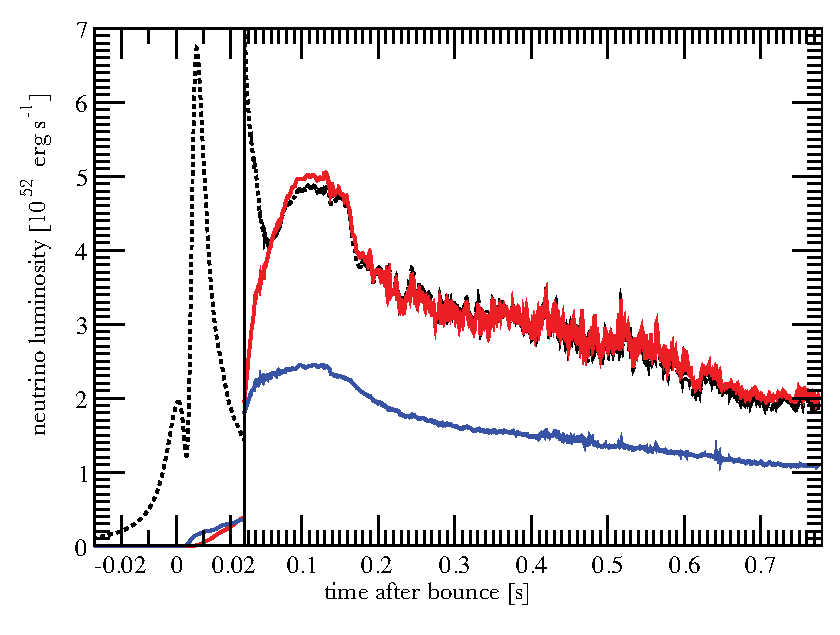
\includegraphics[width=0.8\textwidth]{neutrino_time}
			\caption[Simulated Supernova Neutrino Signal]{\bf Simulated supernova neutrino signal. \rm The simulation of this $15 M_\odot$ star was general relativistic and 2 dimensional. The black lines are for $\HepParticle{\Pnue}{}{}$, the red lines for $\HepParticle{\APnue}{}{}$, and the blue lines for heavier neutrinos $\nu_x$ \cite{Janka2012}. The neutrino flux persists for several tens of seconds and then fades.}
			\label{fig:neutrino_time}
		\end{figure}
		The electron neutrinos are the first to leave the star. These were the result of neutronization of the inner core and were the constituents of the neutrino breakout. This burst is expected to last for a few tens of milliseconds\cite{Scholberg2012}. Neutrinos generated during shock revival are also predominantly electron flavored. The duration of this period is on the order of $\sim\SI{100}{\milli\second}$\cite{Scholberg2012}. At a post-bounce time of $t \gtrsim\SI{100}{\milli\second}$, convective processes in the neutron star increase the flux of heavier neutrino flavors\cite{Janka2012a}. Over the next ten or twenty seconds, the core cools via neutrino emission (\FIG \ref{fig:neutrino_time}). The spectrum of neutrino energies (\FIG \ref{fig:neutrino_fluence}) emitted from the explosion are centered around a value just above \eMeV{10}\cite{cosmology}.

		\begin{figure}[H]
			\centering
			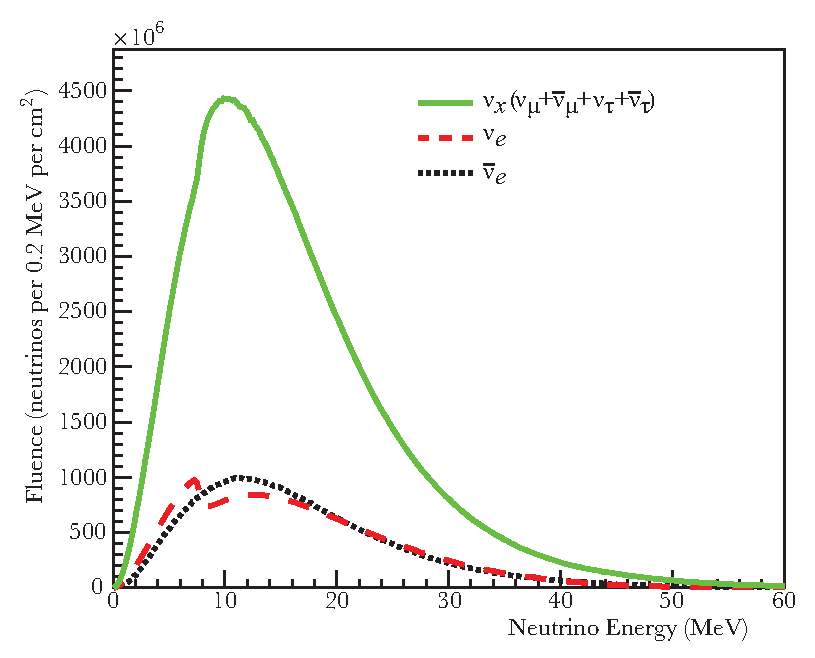
\includegraphics[width=0.9\textwidth]{neutrino_fluence}
			\caption[Simulated Supernova Neutrino Fluence]{\bf Simulated supernova neutrino fluence\rm \cite{Scholberg2012}. \rm The neutrino flux generated by the GVKM model\cite{Gava2009} for a supernova \SI{10}{\kilo\parsec} from Earth was integrated over a period of \SI{10}{\second} to produce this fluence. The energy distribution for all neutrino flavors are centered around $\gtrsim \eMeV{10}$. The model accounts for neutrino-neutrino interactions and dynamic MSW effects, which cause the wobble seen in the \HepParticle{\Pnue}{}{} profile.}
			\label{fig:neutrino_fluence}
		\end{figure}

		It is very helpful that $99\%$ of a supernova's energy is radiated in the form of neutrinos before the outer layers of the star are disrupted. This provides a means of predicting the optical appearance of a supernova. Such an advance warning would be invaluable to astronomy, as it would allow the community to observe a supernova as it happens and better understand the very complex process that surround it (see \CHP \ref{snews_chapter}). Furthermore, the neutrinos themselves can serve as more than just messengers; the properties of the neutrino flux would contain valuable insight to the goings-on in the core during and after collapse.

























%-----------------------------------------------------------------------------
%-----------------------------------------------------------------------------

		% // HALO
			\cleardoublepage
			%-----------------------------------------------------------------------------
%
%          PHYSICS  M.S.     THESIS
%          JUSTIN A. VASEL
%
%          This began as the template offered by the University of Minnesota, 
%          but I've made a few changes here and there...  
%
%          -->  snews.tex
%
%-----------------------------------------------------------------------------


\chapter{The Supernova Early Warning System}
	\label{snews_chapter}
	\vspace{-0.2in}

	\begin{quoting}
		\noindent \large ``Vision is the art of seeing things invisible." \normalsize

		--- Jonathan Swift
	\end{quoting}

	\chapterIntro{L}{ittle is known about the behavior of a star moments from death.} Understanding of main-sequence stellar behavior is always improving thanks to a robust nuclear theory, powerful computational models, and observation. But, after a star moves off of the main sequence conditions inside are harder to predict with any confidence. Perhaps the best example of this are the moments immediately preceding and immediately following the eruptions of large stars. Computational models are always improving, but its very hard to compare them with observations because it is difficult to predict when and where a supernova will occur. 

	The possibility of using the neutrino signal as an advance warning of the photon signal was fully realized with the eruption of SN 1987a, \SI{50}{\kilo\parsec} away in the Large Magellanic Cloud. A handful of neutrino detectors at the time recorded the event. A total of 26 events were observed between Kamiokande-II, IMB, and Baksan over a period of 13 seconds, all with energies $\lesssim$ \nolinebreak \eMeV{40} (\FIG \ref{fig:SN1987curve})\cite{kii1987a,imb_1987a,baksan1987a}.

	\begin{figure}[H]
	\centering
	    \begin{tikzpicture}[scale=1.5]
	    	\pgfplotsset{every axis legend/.append style={
				at={(0.5,1.03)},
				anchor=south}}
		    \begin{axis}[xmin=0,xmax=15,ymin=0,ymax=50,title={},%
		    xlabel={Time (s)}, ylabel={Neutrino energy (MeV)},%
		    legend cell align=left, only marks, legend columns=3, legend style={/tikz/every even column/.append style={column sep=0.5cm}}]
		        \addplot[red,thick,mark=*,/pgfplots/error bars/.cd, x dir=none,y dir=both,y explicit] table[x index=0, y index=1, y error index=2] {./Chapters/Supplementary/k2.dat};
		        \addlegendentry{Kamiokande II}
		        \addplot[blue,thick,mark=square*,/pgfplots/error bars/.cd, x dir=none,y dir=both,y explicit] table[x index=0, y index=1, y error index=2] {./Chapters/Supplementary/imb.dat};
		        \addlegendentry{IMB}
		        \addplot[black,thick,mark=triangle*,/pgfplots/error bars/.cd, x dir=none,y dir=both,y explicit] table[x index=0, y index=1, y error index=2] {./Chapters/Supplementary/baksan.dat};
		        \addlegendentry{Baksan}
		    \end{axis}
	    \end{tikzpicture}
	    \caption[Observed Neutrino Spectrum From SN 1987a]{\bf Observed neutrino spectrum from SN 1987a. \rm Twenty six events were recorded by three separate experiments during a 13-second period. A scintillator detector in Mont Blanc in Italy detected a neutrino signal, but it was not coincident with the other detectors and are not thought to be associated with the supernova\cite{Arnett1989}.} \label{fig:SN1987curve}
	\end{figure}

	The Supernova Early Warning System (SNEWS)\footnote{http://snews.bnl.gov} \cite{Scholberg2008} is hoping to take advantage of the neutrino signal generated during galactic core-collapse supernovae to identify the explosion before the photon signal arrives. SNEWS is a world-wide network of neutrino detectors that will listen for that distinct neutrino signal and alert the astronomical community upon its arrival. Astronomers will only have several hours to prepare their observations. 


	%% SECTION : A WORLD-WIDE NETWORK OF NEUTRINO DETECTORS
	\section{A World-Wide Network of Neutrino Detectors}
	There are at present five neutrino observatories actively participating in SNEWS: IceCube in Antarctica, Borexino and the Large Volume Detector (LVD) in Italy, and Super-Kamiokande (Super-K) and KamLAND in Japan. HALO and a few other experiments like SNO+ in Canada and NO$\nu$A in Minnesota plan to join that list soon. A brief summary of each detector is given in \TAB \ref{table:snews_detectors}.
		\begin{figure}[H]
		\centering
		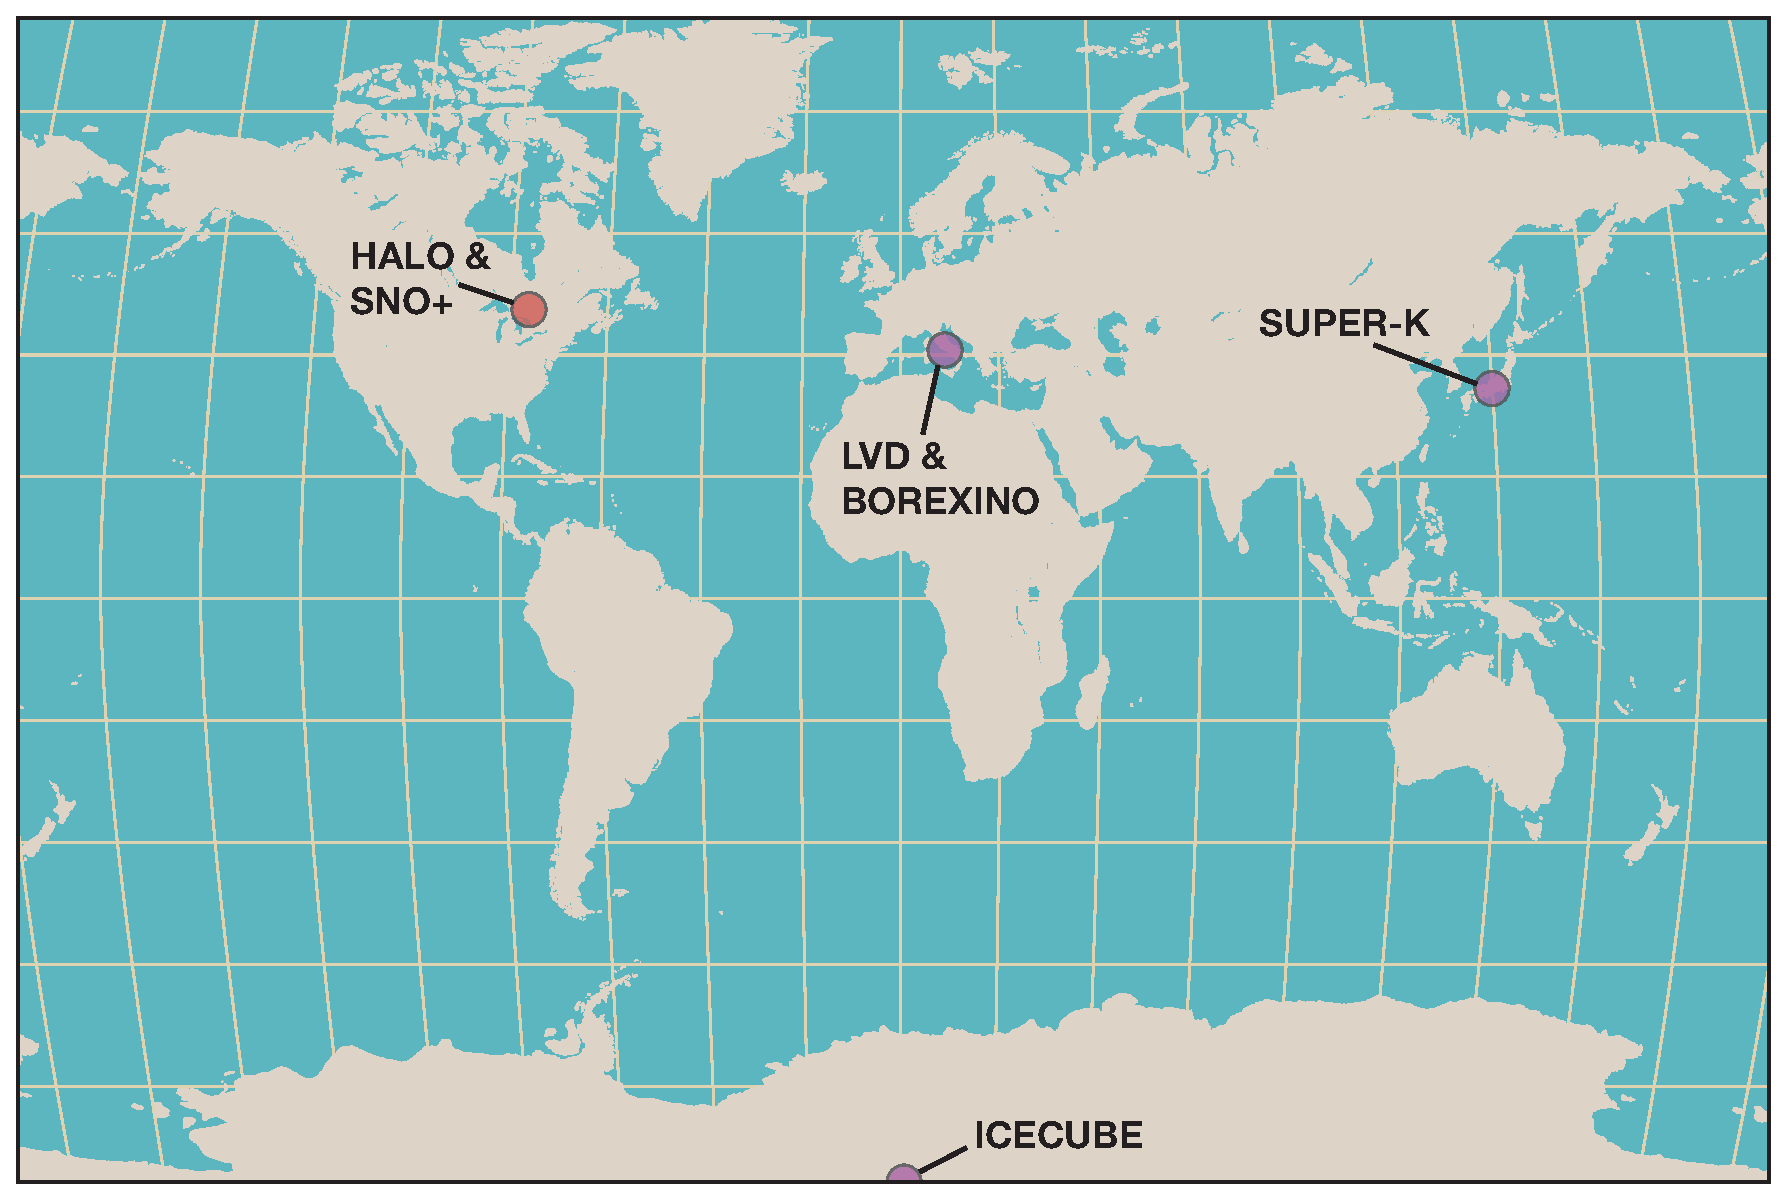
\includegraphics[width=1\textwidth]{snews_map}
		\caption[Map of Observatories Participating in SNEWS]{\bf Map of observatories participating in SNEWS. \rm At present, five observatories are actively participating (purple markers). HALO, SNO+, and NO$\nu$A plan to actively participate once their triggers are in place (red markers).}
		\label{fig:snews_map}
	\end{figure}

	The experiments share a connection to two central servers, one at Brookhaven National Laboratory (BNL) and another at the Istituto Nazionale di Fisica Nucleare in Italy, which functions as a backup in case BNL goes offline. Through automated triggering software, each experiment automatically sends an alert to the central server when it believes it detected a supernova neutrino signal. If the server receives several coincident alerts, it sends the warning out to the SNEWS membership via a PGP encrypted email. 

	\begin{table}[H]
		\centering
		\caption[Summary of SNEWS Detectors]{A summary of SNEWS-affiliated detectors and their attributes\cite{Antonioli2004}.}
		\label{table:snews_detectors}
			\begin{tabular}{lcccc}
				\toprule
				Detector & Type & Mass (kton) & Location & Status \\
				\midrule
				IceCube & H$_2$O (ice) Cherenkov & -- & Anarctica & Running \\
				Borexino & Liquid Scintillator & 0.30 & Italy & Running \\
				LVD & Liquid Scintillator & 1 & Italy & Running \\
				Super-K & H$_2$O Cherenkov 	& 32 & Japan & Running \\
				HALO & High-Z (Pb) & 0.076 & Canada & In Development \\
				SNO+ & Liquid Scintillator & 0.78 & Canada & In Development \\
				\bottomrule
			\end{tabular}
	\end{table}


	%% SECTION : THE THREE P'S
	\section{The Three P's}
	In order for SNEWS to be reliable and successful, it has to adhere to ``the three P's":

	\subsection*{Prompt}
	The prompt neutrino signal may only precede the photon signal by hours or less. It is essential that SNEWS works quickly to get the word out once the neutrino signal is detected. To achieve this, the system is automated at both the detector end and the server end. Each experiment is responsible for developing its own software triggers that alert SNEWS when a supernova candidate is detected. 

	\subsection*{Pointing}
	Knowing that a supernova is about to become visible is great. What's better is knowing where to look. Detecting the directionality of incoming neutrinos is notoriously difficult. Many neutral and charged current interactions are useless because their products are nucleons or leptons whose directions are independent of that of the neutrino. However, elastic scattering between neutrinos and electrons ($\HepProcess{\HepParticle{\Pneutrino}{}{} + \HepParticle{\Pelectron}{}{} \to \HepParticle{\Pneutrino}{}{} + \HepParticle{\Pelectron}{}{}}$), which is a neutral current process, is currently the best method because the momentum transfered to the electron points back to the direction of the incoming neutrino. Super-Kamiokande is currently the only SNEWS observatory that can provide pointing information. For a supernova at a distance of \SI{10}{\kilo\parsec} from Earth, Super-K can point with an accuracy of about \ang{7.8} if an isotropic background is present. If the background can be accounted for with neutron tagging, the accuracy improves to about \ang{3.2}\cite{Tomas2003}. Triangulation between detectors around the world is technically possible, but currently the statistics associated with interactions make it too difficult. It has been proposed that the next generation of high-statistics neutrino observatories (eg. Hyper-Kamiokande) may be able to use triangulation to determine a rough location in the sky\cite{Muhlbeier2013}.

	%\vspace{0.5in}
	\subsection*{Positive}
	\label{sec:snews_positive}

	\begin{wrapfigure}{r}{0.68\textwidth}
		\vspace{-0.9in}
		\centering
		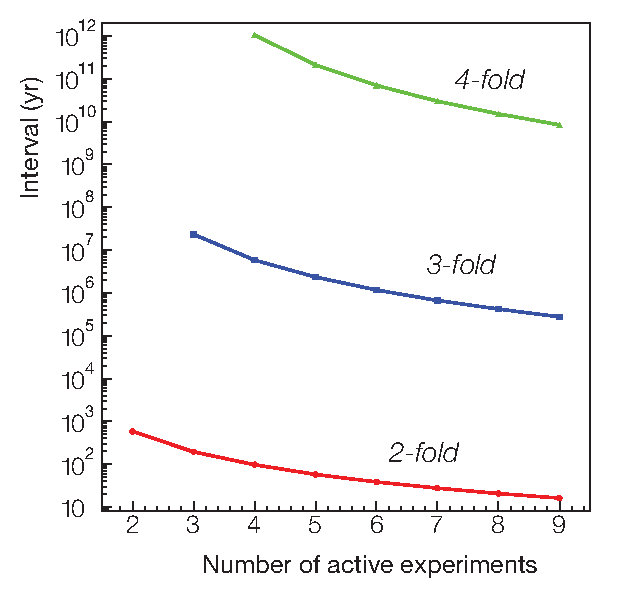
\includegraphics[width=0.68\textwidth]{coincidence}
		\caption[SNEWS Rate of Accidental Alerts]{\bf SNEWS rate of accidental alerts.\rm The average interval between false-alarms is modeled to first order as a Poisson process parameterized by the number of required coincidences in a 10 second window and the number of active experiments\cite{Antonioli2004}.}
		\label{fig:coincidence}
		\vspace{0.0in}
	\end{wrapfigure}


	To ensure that a SNEWS alert is taken seriously, the false-alarm rate of SNEWS must be very low. SNEWS aims for a false-alarm rate of fewer than one per century. To achieve this, SNEWS requires that each experiment has a false-alarm rate of less than once per week and that at least two detectors send an alert within ten seconds of each other. This 2-fold coincidence between detectors ensures the once-per-century threshold can be achieved, but only with three actively participating experiments. If more than three experiments are participating, the coincidence between detectors must be at least 3-fold if each detector is to maintain a once-per-week false alarm rate pre-coincidence (\FIG \ref{fig:coincidence}).


	%% SECTION : ALERTING THE ASTRONOMICAL COMMUNITY
	\section{Alerting the Astronomical Community}
	Each experiment participating in SNEWS is responsible for implementing an automated supernova trigger with the certainty detailed in the previous section. When an experiment's trigger is activated, the experiment will send an alarm datagram to the ``coincidence server'' in Brookhaven National Laboratory. The coincidence server then scrutinizes the datagram and listens for coincident alarms from other experiments. A 2-fold coincidence within 10 seconds is required to trigger an automated alert. If the coincidence criterion is not met, an individual alert can be sent if the experiment confirms the signal is not noise, otherwise the datagram is discarded and SNEWS returns to waiting for alarms (\FIG \ref{fig:flowchart}).

	If the coincidence criterion is met, then SNEWS will issue either a GOLD or SILVER alert, depending the quality of the alarm received. Besides coincidence, for a GOLD alarm to be issued at least two of the experiments involved must be a physically separated laboratories. Furthermore two or more of the alarms received must be flagged as ``GOOD''. This means that the alarm was received while the experiments were operating under normal conditions, rather than operating during maintenance or callibrtion, for example. Finally, at least two of the experiments involved must have had an acceptable false-alarm rate of \SI[mode=text]{1}{week^{-1}} during the past time intervals $\{T_i\} = \{\SI[mode=text]{10}{minutes}, \SI[mode=text]{1}{hour}, \SI[mode=text]{10}{hours}, \SI[mode=text]{1}{day}, \SI[mode=text]{3}{days}, \SI[mode=text]{1}{week}, \SI[mode=text]{1}{month}\}$.

	If a coincident alarm fails to meet all these criteria, the alert will be demoted to SILVER. A SILVER alert only gets issued to experimenters, not the general public. In this case experimenters must personally check their data and decide if it is a suitable supernova candidate. If so, the experimenters send an OVERRIDE packet to the server and SNEWS promotes the alert to GOLD. A GOLD alert is issued to experimenters and the public. Again, the experimenters must hand-check their data. If through this checking it is discovered that it was a false alarm, a retraction is issued to the mailing lists and on the SNEWS web page.

	\begin{figure}[H]
		\centering
		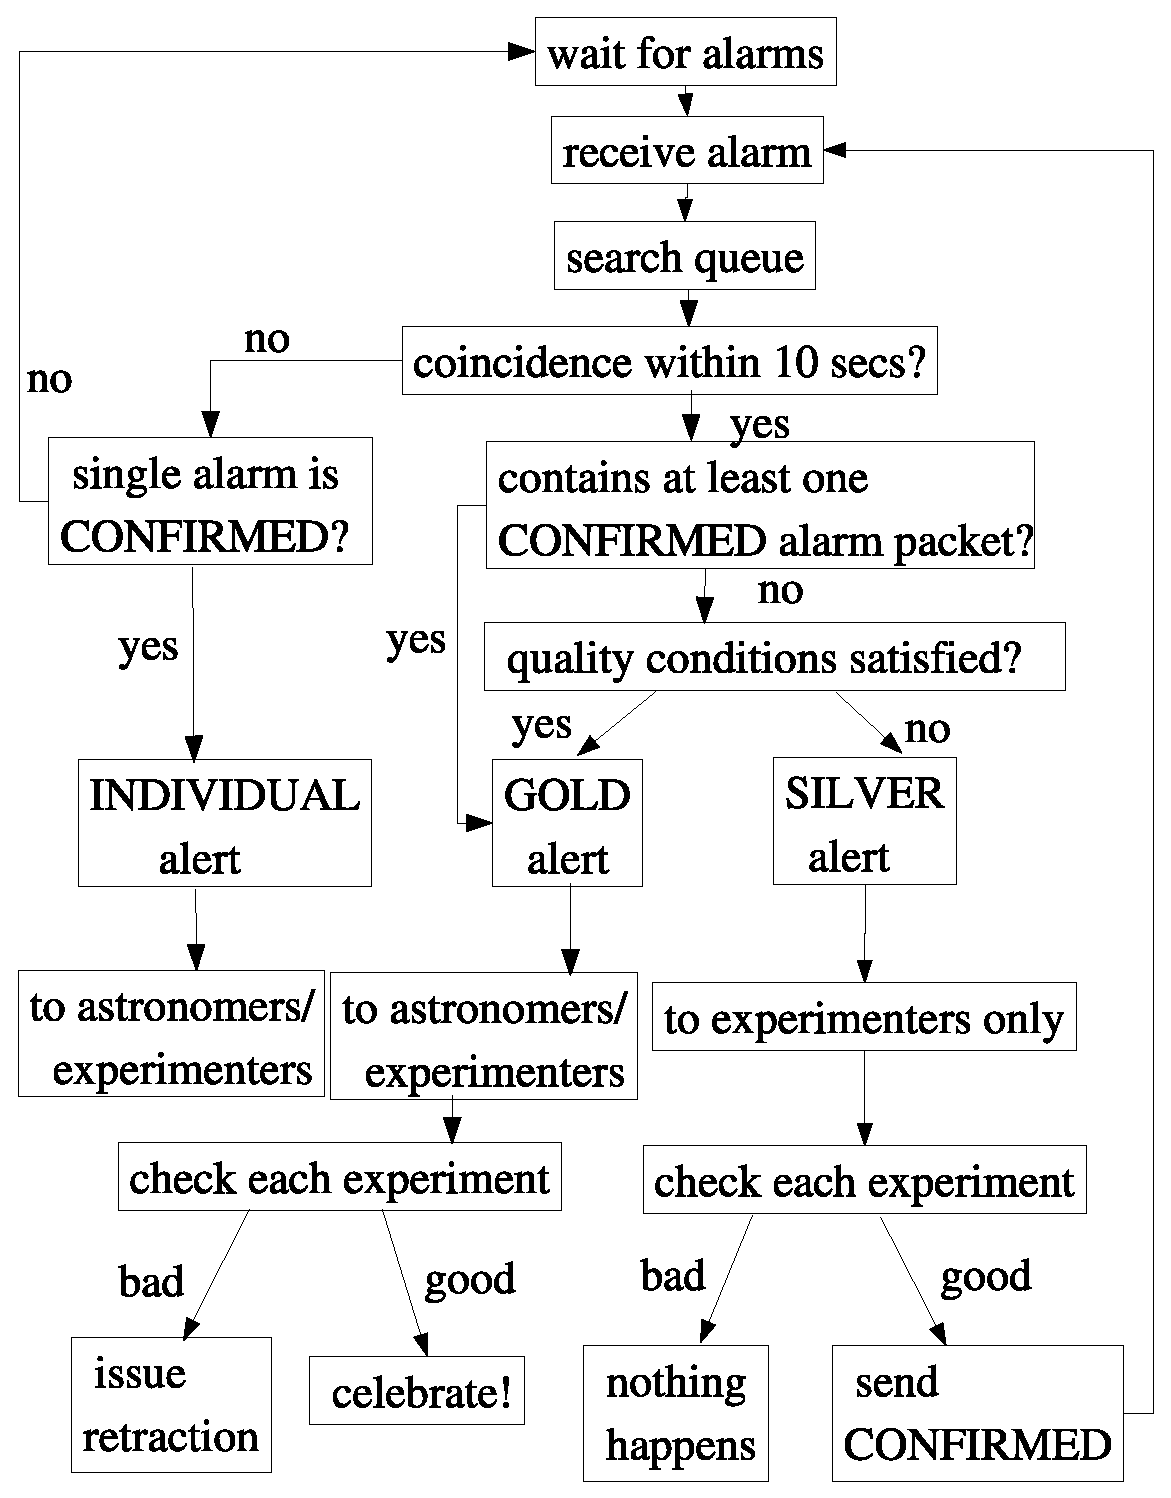
\includegraphics[width=0.68\textwidth]{snews_flowchart}
		\caption[SNEWS Flowchart]{\bf SNEWS alert flowchart\rm\cite{Scholberg2008}. This algorithm runs on the SNEWS coincidence server at Brookhaven National Laboratory, and discriminates against alarms to determine their candidacy as a supernova event.}
		\label{fig:flowchart}
	\end{figure}

	The intended subscribers of the SNEWS service are astronomers, although anybody who would like to receive alerts can sign up.\footnote{Join the mailing list: http://snews.bnl.gov/alert.html} An alert sent to the community will contain information about the time of the event and an approximate location in the sky bounded by an error box. This pointing information may not be included with any alert; it depends on which experiments can provide such information and whether they were involved in the coincidence. The neutrino detectors are the ear, but the optical telescopes are the eyes. The amateur astronomers---being skilled, enthusiastic, and well-equipped---are well suited for this task.

	In 2003, a test alert was issued to observe the system in action. The asteroid Vesta was selected as the test target and the position with a 13 degree uncertainty was distributed to the mailing list. Amateur astronomers world-wide submitted 83 responses, of which six had successfully identified the target\cite{Antonioli2004}. The system worked.

%-----------------------------------------------------------------------------
%-----------------------------------------------------------------------------
			
			\cleardoublepage
			%-----------------------------------------------------------------------------
%
%          PHYSICS  M.S.     THESIS
%          JUSTIN A. VASEL
%
%          This began as the template offered by the University of Minnesota, 
%          but I've made a few changes here and there...  
%
%          -->  halo.tex
%
%-----------------------------------------------------------------------------


\chapter{Helium and Lead Observatory}
	\label{halo_chapter}

	\begin{quoting}
		\noindent \large ``Astronomically Patient" \normalsize

		--- The HALO Collaboration
	\end{quoting}

	\chapterIntro{B}{uried 6,800 feet below ground,} SNOLAB is the deepest laboratory in the world. SNOLAB is located near Sudbury, Ontario, Canada in the Vale Creighton Mine. Originally, the laboratory consisted of just one experiment, the Sudbury Neutrino Observatory (SNO). Due to the success of SNO in shedding light on the solar neutrino problem, the laboratory expanded and now is home to a handful of neutrino and dark matter experiments. The Helium and Lead Observatory (HALO) is one of the experiments that calls SNOLAB its home. 

	The HALO experiment is currently in the final stages of development. When it is complete, HALO will continuously search for the distinct neutrino signal produced during a galactic supernova as a member of SNEWS. HALO is unique in that it is the only neutrino experiment whose primary objective is to detect supernova neutrinos.

	\begin{figure}[H]
		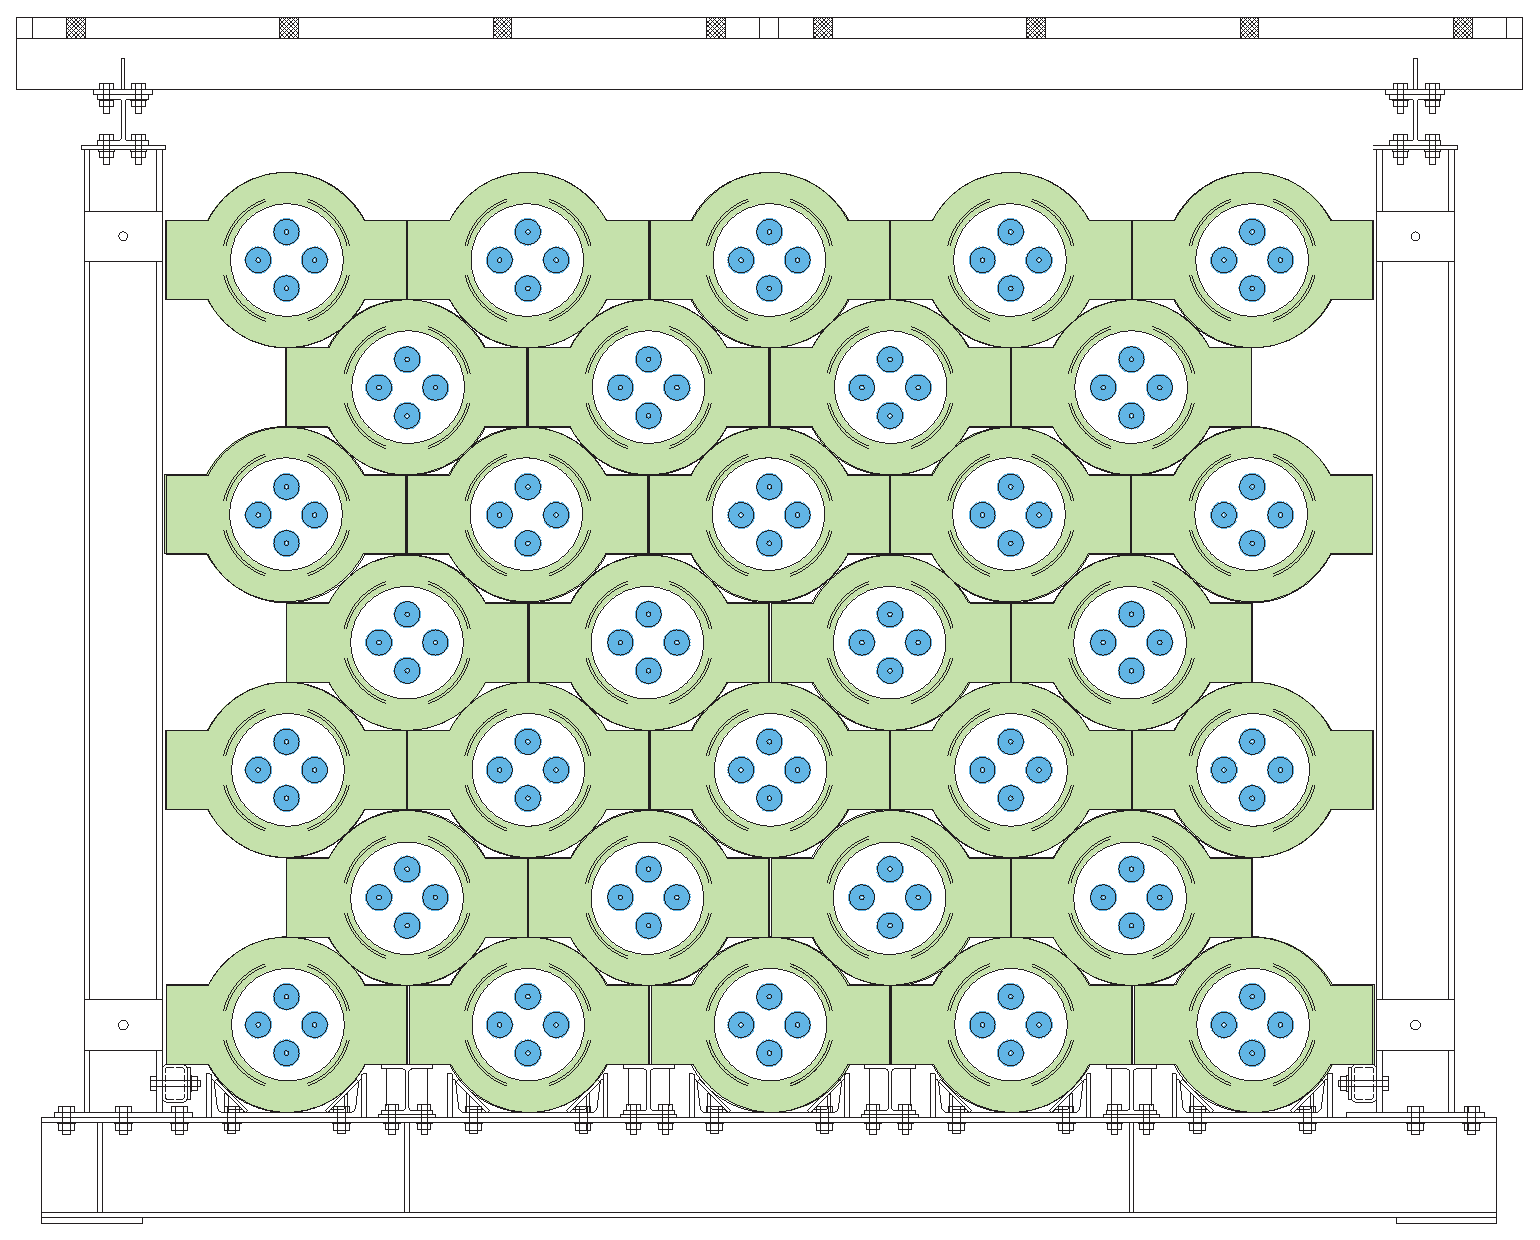
\includegraphics[width=\textwidth]{halo_diagram}
		\caption[The HALO Detector]{\bf Schematic of the HALO detector design (Front View). \rm The lead blocks (stacked objects, shaded green) are the site of neutrino interactions. The products of those interactions, neutrons, travel into the \he proportional counters (four circles contained within each lead block, shaded blue) and are captured on \he. The structure is \SI{2.4}{\metre} tall.}
		\label{fig:halo}
	\end{figure}

	The HALO detector consists of \ \SI[mode=text]{76}{tons} of lead and 128 \he neutron detectors. The lead serves as the interaction medium and is sectioned in blocks. Each block of lead has a bore through the middle of it within which sit four \he neutron detectors \nolinebreak (\FIG \ref{fig:halo}). The 864 lead blocks used in HALO are stacked in such a way that every bore extends \SI{3}{\metre} in length. Most of the \he detectors are also \SI{3}{\metre} long. However, there were not enough detectors of that length to fill up all 128 positions. Several \SI{2.5}{\metre} long detectors were used to fill the extra space.

	Because galactic supernovae only occur two or three times each century\footnote{Despite this predicted occurrence rate, the most recently observed supernova within the Milky Way was spotted by Johannes Kepler in 1604.}\cite{sn_rates}, HALO is designed with longevity in mind. Once completed, the experiment will be highly automated and relatively inexpensive to maintain, allowing it to remain in operation for decades. 



	%% SECTION : LEAD AS AN INTERACTION MEDIUM
	\section{Lead as a Interaction Medium}

		HALO is the only neutrino experiment that uses lead as an interaction medium. Lead was chosen because it was economical, available, and efficiently delivers neutrino-induced neutrons to the \he neutron counters in which detection actually occurs. Lead has a relatively high neutrino interaction cross section which results in the production of neutrons\cite{Engel2003}. These interactions (\FIG \ref{fig:sensitivities}) are neutral current (NC) interactions, which are moderated by the $\HepParticle{\PZzero}{}{}$ boson (\EQ \ref{eq:nc}), or charged current (CC) interactions, which are moderated by the $\HepParticle{\PWpm}{}{}$ bosons (\EQS \nolinebreak \ref{eq:nue_cc} \& \nolinebreak \ref{eq:nue_bar_cc}).
			\begin{align}
				\quad \textbf{Neutral Current} \qquad &\HepProcess{\HepParticle{\Pneutrino}{}{} + \text{Pb} \to \HepParticle{\Pneutrino}{}{*} + \text{Pb}^*} \label{eq:nc} \\
				\quad \textbf{$\HepParticle{\Pnue}{}{}$ Charged Current} \qquad &\HepProcess{\HepParticle{\Pnue}{}{} + \text{Pb} \to \HepParticle{\Pelectron}{}{} + \text{Bi}^*} \label{eq:nue_cc} \\
				\quad \textbf{$\HepParticle{\APnue}{}{}$ Charged Current} \qquad &\HepProcess{\HepParticle{\Pnue}{}{} + \HepParticle{\Pproton}{}{} \to \HepParticle{\Ppositron}{}{} + \HepParticle{\Pneutron}{}{}} \label{eq:nue_bar_cc}
			\end{align}
			In NC interactions, a neutrino of any flavor strikes a lead nucleus and excites it. When the nucleus de-excites, zero, one, or two neutrons are produced ($\HepProcess{\text{Pb}^* \to \text{Pb} + \HepParticle{\Pphoton}{}{} + \text{neutrons}}$). In $\HepParticle{\Pnue}{}{}$ CC interactions, an electron neutrino interacts with a neutron in the lead nucleus, producing an electron and bismuth in an excited state. Again, the nucleus de-excites and produces zero, one, or two neutrons ($\HepProcess{\text{Bi}^* \to \text{Bi} + \HepParticle{\Pphoton}{}{} + \text{neutrons}}$).

			\begin{figure}[H]
				
\includegraphics[width=\textwidth]{total}
				\vspace{-0.3in}
				\caption[Neutrino Detector Sensitivities]{\bf Neutrino detector sensitivities. \rm Different neutrino interaction materials have different neutrino flavor sensitivities. This figure shows which interaction channels appear as a proportion of the total neutrino signal for popular interaction media. Since HALO is the first experiment to lead as an interaction medium, it will offer unique insight into the $\HepParticle{\Pnue}{}{}$ charged current channel.}
				\label{fig:sensitivities}
			\end{figure}
			\vspace{-0.1in}
		Scaling from the calculations of Engel, McLaughlin, and Volpe\cite{Engel2003}, a supernova \SI{10}{\kilo\parsec} from Earth would produce 29 single neutrons and 18 double neutrons from the charged current channel, and 8 single neutrons and 6 double neutrons from the neutral current channel\cite{Shantz2010}. Not all of these events will be detected, however. HALO's detection efficiency is estimated to be $\sim 40\%$\cite{Shantz2010,Scholberg2011}. The efficiency will be more accurately known after improvements have been made to the detector Monte Carlo simulation.

		The third possible interaction, $\HepParticle{\APnue}{}{}$ CC, is highly suppressed due to ``Pauli blocking.'' The excess of neutrons in lead makes it less likely that neutron will be produced because many of the low-energy states are already filled, and neutrons are fermionic particles that are subject to the Pauli exclusion principle. 

		The lead blocks were originally used in the Deep River cosmic ray monitoring station\cite{Shantz2010}. The lead is stacked in alternating rows of four and five (\FIG \ref{fig:halo}) and each row runs 3 meters deep. This geometry was chosen to maximize the number of lead blocks used while being confined to the relatively small space that HALO is given in SNOLAB. HALO makes use of 76 tons of lead; 864 blocks in total. The lead blocks were painted to minimize health risks associated with exposure to lead and to minimize contamination of the SNOLAB environment. The paint was meticulously chosen based on several factors, including its resistance to peel or rust, its neutron-capture cross section, and its containment of radioactive isotopes that could increase background noise in the detector\cite{Shantz2010}.


	%% SECTION : 3HE PROPORTIONAL COUNTERS
		\section{\he Proportional Counters}

		\begin{figure}[H]
			\includegraphics[width=\textwidth]{ncd}
			\caption[Technical Diagram of \he Proportional Counter]{\bf Technical diagram of \he proportional counter\rm \cite{Schumaker2010}. The counters were originally used in Phase III of the SNO experiment, but have been refitted with new endcaps for use in HALO.}
			\label{fig:ncd}
		\end{figure}

		The neutrons produced from nuclear de-excitation of either lead or bismuth pass into one of the 128 proportional detectors (\FIG \ref{fig:ncd}) which are filled with a gaseous mixture of \he and CF$_4$ (85/15 by pressure) at a pressure of \SI[mode=text]{2.5}{atm}. The neutrons are captured on \he shortly after entering the tube by the following reaction:
		\begin{equation}
			\HepProcess{^3\text{He} + \HepParticle{\Pneutron}{}{} \to \HepParticle{\Pproton}{}{} + {}^3\text{H} + \ekeV{764}}
		\end{equation}
		Of the \ekeV{764} released from the reaction, \ekeV{573} is the kinetic energy of the proton and \ekeV{191} is the kinetic energy of the triton. The production of these charged particles (\FIG \ref{fig:capture}) ionizes the nearby gas, producing ion pairs that are accelerated in opposite directions by a potential difference between a coaxial anode and cathode. The electric field near the anode is strong enough to allow secondary ionization of the surrounding gas by the accelerating electrons. This produces a cascade of ionization that is ultimately collected on the anode. The amount of charge collected at the anode is proportional to the original number of ion pairs. 

		\begin{figure}[H]
			\centering
			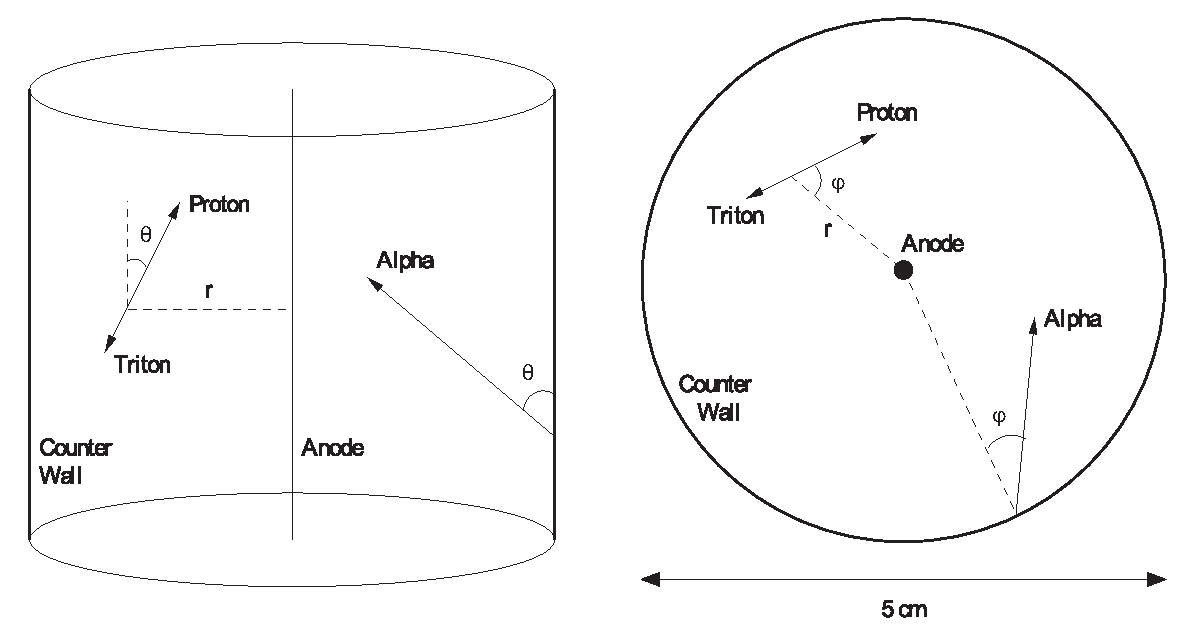
\includegraphics[width=0.9\textwidth]{capture}
			\caption[\he Neutron Capture Schematic]{\bf \he Neutron capture schematic\rm \cite{Search2011}. The proton-triton pair are produced and move in opposite directions. The proton and triton peaks may be separated in time by an amount determined by their orientation in the counter.}
			\label{fig:capture}
		\end{figure}

		The spectrum of neutron energies does not have a single sharp peak at \ekeV{764}, however. Instead, the spectrum has two distinct shoulders to the left of the peak (\FIG \nolinebreak \ref{fig:neutron_spectrum}). These shoulders are artifacts of the ``wall effect.'' The wall effect occurs when neutron capture happens very close to the detector wall. When the proton and triton are created, one of them may collide with the wall of the detector or be absorbed by it entirely, reducing the total kinetic energy detected by the counter.

		\begin{figure}[H]
			\centering
			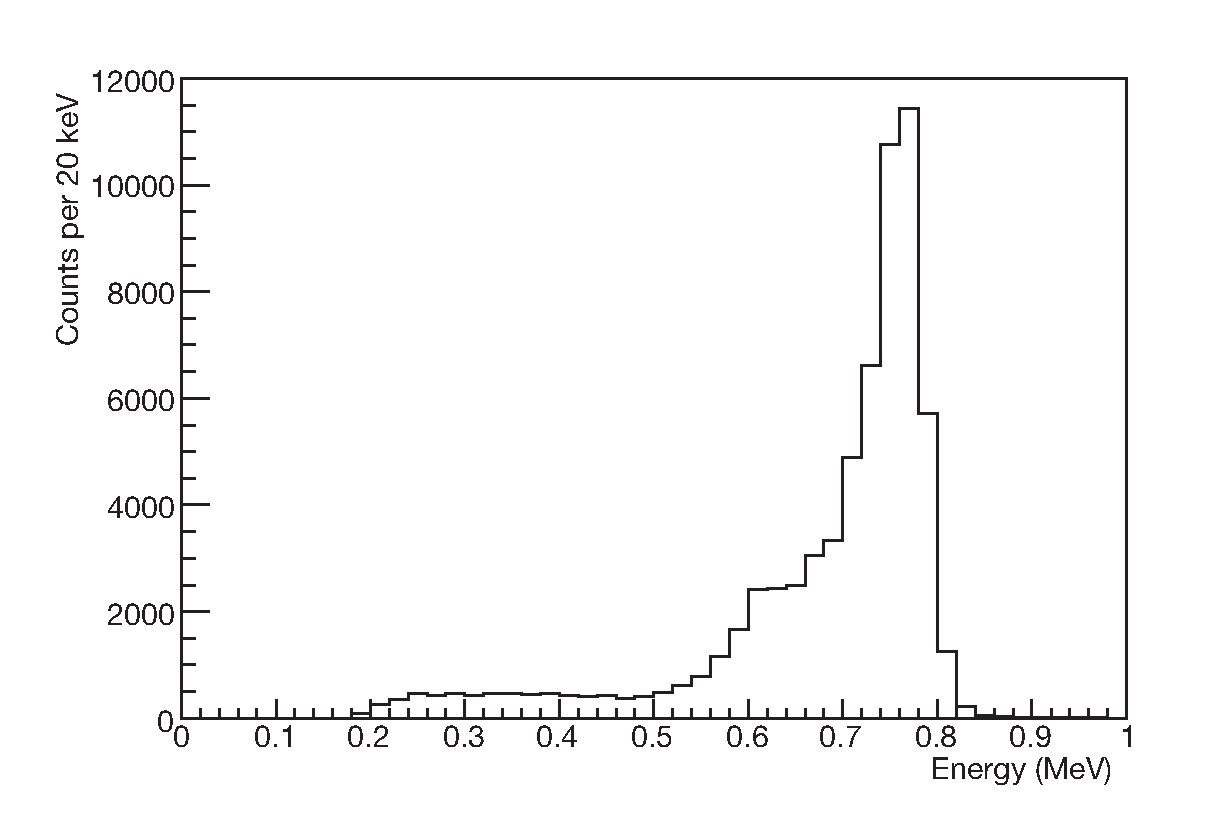
\includegraphics[width=0.9\textwidth]{neutron_spectrum}
			\caption[Example Neutron-Capture Spectrum]{\bf \he neutron-capture spectrum from $^{24}$Na calibration\rm \cite{Search2011}. The neutron peak is clearly located at \ekeV{764}, but there also exist shoulders that terminate at \ekeV{573} and \ekeV{191} due to some of the triton's or proton's energy (respectively) being lost due to collisions with the walls of the counter.}
			\label{fig:neutron_spectrum}
		\end{figure}


	%% SECTION : NEUTRON BACKGROUNDS AND NOISE
	\section{Neutron Backgrounds and Noise}
	\label{sec:noise}

		SNOLAB is better than any other laboratory when it comes to shielding. The \SI[mode=text]{6800}{feet} of rock that sit above it is the equivalent of \SI{6000}{\meter} of water. That notwithstanding, there is still background flux of both fast and thermal neutrons produced by radioactive decays and cosmic ray muon interactions within the surround rock. The flux of thermal and fast neutrons in SNOLAB has been measured to be \SI[mode=text]{4100}{neutrons.m^{-2}.day^{-1}} and \SI[mode=text]{4000}{neutrons.m^{-2}.day^{-1}} respectively\cite{handbook}. 

		To ensure that HALO will maintain the false-alarm rate required for participation in SNEWS (see \SEC \ref{sec:snews_positive}), shielding has been placed around the detector to block as much of the neutron background as possible. Hydrogen makes a great neutron shield because its small mass makes it effective at stealing momentum from fast neutrons, slowing them down. Capture of the thermal neutrons by hydrogen can then occur. The shielding is in the form of water boxes that have a volume of \SI[mode=text]{1}{ft^3}. The boxes have a bladder inside to hold the water. The empty spaces in the box that are not occupied by the water bladder are filled with polystyrene beads. These boxes are placed along the top, back, and sides of the detector. Soon water boxes will cover up the front face of the detector as well.
	 
		The proportional counters are very effective as long as ionization is induced by neutron capture events only. Collisions within\he gas can excite molecules without ionizing them, leading to the emission of a photon when the molecule de-excites. The photons can then go on to cause ionization elsewhere in the detector. This is the reason for the \he/CF$_4$ mixture. The CF$_4$ provides stopping power for ionizing particles, substantially reducing the effect.

		The outer shell of the\he counter is composed of ultra-pure nickel. The walls are only \SI{380}{\micron} thick and were produced in a uniform way through the process of chemical vapor deposition. Despite the purity of the detector material, there are trace amounts of radioactive nuclei that contribute to noise in the signal. The most common byproduct of radioactive decays are alpha particles. The alphas can interact with other elements resulting in the production of a neutron. Fortunately, alpha particles have charge and are very heavy, so they have a very short range. This prevents them in many cases from arriving at the detector wall with sufficient energy to initiate radioactive decay. 

		The few neutrons that are produced by interactions with alpha particles have energies that are a couple tens of \eMeV{}, making them indistinguishable from neutrons produced by supernova neutrino interactions. A study of these alpha backgrounds found that the rate of neutron-producing alphas was $21.9^{+1.1}_{-1.0}$ per day and is considered negligible \cite{Shantz2010}. 

		Gamma rays are another source of noise and are produced through nuclear decays of uranium and thorium found in the paint that coats the lead blocks. Uranium and thorium decay via $\alpha$ or $\beta$ emission, but the decay of daughter nuclei can produce gammas. The gammas then can interact with electrons via Compton scattering and induce ionization within the \he detectors. Multiple scattering effects may imbue the electrons with enough energy to survive being cut by detector electronics, resulting in the false count of a neutron. Simulations\cite{Shantz2010} and HALO data show that the energy of these gamma-induced counts tends to be less than a few \eMeV{}, making them easily distinguishable from the neutrino-induced neutron signal.


 	%% SECTION : DETECTOR ELECTRONICS AND DATA FLOW
	\section{Detector Electronics and Data Acquisition}
	\label{sec:electronics}
	
		The HALO detector and its associated hardware is controlled by a software application called ORCA. This software will be described in greater detail in \SEC \ref{sec:orca_development}. For now, I will briefly describe the electronics configuration of the experiment. The flow of data is illustrated in \FIG \ref{fig:electronics}. The charge collected by the \he counter anode is converted into a voltage and stepped up to a higher voltage by a preamplifier (preamp). The 128 detectors are connected in pairs, so only 64 preamps are used. The signal from the preamps is read into one of 8 shaper ADC boards, each having 8 channels. The shaper ADCs discriminate the signal according to thresholds that are set by the experimenters and then digitize the signal.

		The shaper cards then pass the digitized signal to a single board computer (SBC) running Linux through a common VME bus. The SBC then passes the data to the ORCA software running on the DAQ computer. The HV on the preamps is controlled through ORCA. A HV feedback ADC is used to continuously monitor the voltage. 

		A pulse distribution system has been implemented recently (not shown in \FIG \ref{fig:electronics}). The system allows experimenters to send a simulated pulse into the preamps as a means of testing their response. The system can also be used to characterize the response of the detector. For example, the pulser was recently used to measure the time delay between the recording of events that occurred in separate detectors simultaneously\cite{pulser_timing}. Pulses are timestamped by the trigger card. Currently, the times are provided by an NTP (Network Time Protocol) server on a local Linux box. To produce more accurate timestamps, the collaboration is currently working with SNOLAB to acquire GPS NTP servers. 
		\begin{figure}[H]
			\includegraphics[width=\textwidth]{electronics}
			\caption[HALO Electronics]{\bf HALO electronics diagram. \rm The \he detectors are joined in pairs and connected to 64 preamps where the charge collected at the \he counter anode is converted into a high voltage (HV). The signal is sent to shaper ADC boards which digitize and integrate the current. The digitized signal is then sent to a Linux single board computer (SBC) and is passed to the ORCA software that runs on the DAQ computer. The HV system is controlled by the ORCA software. A HV ADC is used as a feedback mechanism to monitor the voltages in nearly-real-time. A pulse distribution (not shown) has been implemented to allow the injection of simulated pulse signals into the preamps as a way to test their response.}
			\label{fig:electronics}
		\end{figure}


%-----------------------------------------------------------------------------
%-----------------------------------------------------------------------------
			
			\cleardoublepage
			%-----------------------------------------------------------------------------
%
%          PHYSICS  M.S.     THESIS
%          JUSTIN A. VASEL
%
%          This began as the template offered by the University of Minnesota, 
%          but I've made a few changes here and there...  
%
%          -->  halo2.tex
%
%-----------------------------------------------------------------------------


\chapter{The Road to Full Operation}
	\label{halo2_chapter}

	\begin{quoting}
		\noindent \large ``For tomorrow belongs to the people who prepare for it today." \normalsize

		--- African Proverb
	\end{quoting}

	\chapterIntro{I}{arrived at SNOLAB to begin work on HALO in July of 2012.} Construction of the detector hardware had finished not long before that and the detector had been running and collecting data since May of 2012. However, HALO was far from being ready to do its job. Many vital components were missing: SNEWS alert triggers were not developed, hardware redundancy was not in place, there was no way to remotely monitor the hardware, and the detector had not yet been calibrated. 

	My work at HALO was not singularly data analysis nor theoretical research nor computer simulation. My contribution to the experiment was more vague and arguably more involved: to help the collaboration move through this laundry list of tasks in a timely manner so that HALO will be ready to serve its purpose before the next galactic supernova occurs. In this chapter, I will discuss my involvement in preparing the Helium and Lead Observatory for full operation.

	
	%% SECTION : INDENTIFYING FAULTY 3HE COUNTERS
	\section{Identifying Faulty{}\he Counters}
		As mentioned in \CHP \ref{halo_chapter}, the{}\he proportional counters were donated to HALO by the decommissioned SNO experiment. Only 128 counters are required for HALO, which left us with a couple dozen extra to be kept on reserve in case a counter in the detector for whatever reason needs to be replaced. The neutron spectrum for each counter currently in the detector had been carefully examined to ensure the active counters were behaving as expected, but the extra counters had not yet been so thoroughly vetted. It was known that some of the counters were filled with $^4$He gas, which cannot be used in the detection of neutrons. The SNO experiment used these as a control group and they got mixed in with the{}\he counters when they were delivered to HALO. 

		To identify the $^4$He counters in the group and to ensure that the{}\he counters were behaving normally, we tested each of them by collecting and examining their neutron spectrum. To avoid disrupting any of the 128 active counters in the detector during testing, we ran wiring from the storage rack to the rest of the hardware. This allowed us to test four counters at a time while the rest of the detector ran normally.

		Most counters were allowed to accumulate data for several days before inspection. A healthy{}\he counter displayed a statistically significant neutron peak located near an ADC value of 1,000\footnote{At this point, the arbitrary ADC value scale for energy had not been mapped to keV. Such a mapping depends on the peculiarities of the{}\he counter, the gains within it, and thresholds applied to it. An algorithm to perform this conversion for each counter is currently in development.} and a tall and sharp gamma peak at very low energies (\FIG \ref{fig:halo_neutron_spectra}, left). An unhealthy{}\he counter may have a broadened neutron peak or other strange artifacts in the spectrum (\FIG \ref{fig:halo_neutron_spectra}, center). A $^4$He counter would simply not have the neutron peak (\FIG \ref{fig:halo_neutron_spectra}, right).
		\begin{figure}[H]
			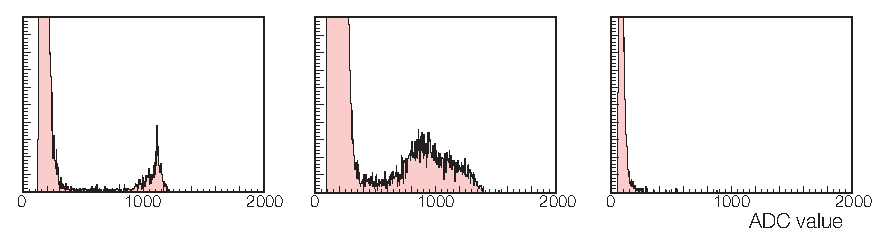
\includegraphics[width=\textwidth]{halo_neutron_spectra}
			\caption[Neutron Counter Response]{\bf Neutron counter response. \rm A healthy{}\he counter \emph{(left)} exhibits a sharp neutron peak and a gamma peak. An unhealthy{}\he counter \emph{(center)} also has a gamma peak, but may show a broadened neutron peak or other obscure features. A $^4$He counter \emph{(right)} features a gamma peak, but no neutron peak.}
		\label{fig:halo_neutron_spectra}
		\end{figure}

		The $^4$He counters are not completely useless to the experiment, however. As discussed in \SEC \ref{sec:noise}, gamma rays produced by the nuclear decay of uranium and thorium daughters in the lead paint can Compton scatter with electrons in the tubes and ionize the surrounding gas. There is no neutron capture processed involved in that case, so both \he and $^4$He counters can detect gamma rays. These counters may be used to study the gamma backgrounds in an effort to separate them from the neutron peaks in the \he counters. 

		After characterization, we identified both healthy and unhealthy{}\he counters and the $^4$He counters. A \he counter with a gas leak will experience either a decrease or increase in gain, depending on how much gas has leaked, and manifest itself as a distorted neutron spectrum. We suspected that any unhealthy spectra we found would be due to such a leak, but after finding several of these, we began to wonder if there was another explanation. It was a symptom worthy of further investigation, in case it represented a larger problem that could affect healthy{}\he detectors down the road.

		It was suggested that perhaps the electrical connection between the anode wire and the endcap that connects it to the high voltage was not sound. The endcaps connect to the anode wire through a small metal spring. At the end of the spring is a ball that fits into a socket at the end of the anode wire. We imagined two scenarios that might degrade the electrical connection: the ball on the spring did not fit into the socket and is instead resting on the side of the anode wire; or the spring has lost compression over time and is no longer making firm electrical contact.

		To test these ideas, we began removing endcaps from the detectors in question and examining the connections. There was no evidence of any of the springs being bent, but the possibility of them having lost sufficient compression to provide a good electrical contact was still plausible. We placed a small dab of conductive grease to the end of the spring ball to provide a strong electrical pathway even if ball and socket were only barely touching. 

		This did not make a difference; the spectra still appeared deformed. Since we tried improving the connection with conductive grease, others have attempted to measure how the spring compression changes over time. They found that the springs do tend to loose compression very quickly. A spring compressed by \SI{4}{\milli\metre} lost much of its compression within the first few minutes and approached a value of \SI{2}{\milli\metre} after a few hours. The manufacturer claims that \SI{2}{\milli\metre} is the amount of compression needed to make a strong electrical contact, so these results initially were not too concerning. However, over a longer time scale of about a week, the springs lost an addition \SI{0.5}{\milli\metre} of compression\cite{spring_test}. It is not clear whether this is the cause of the deformed neutron spectra, but it will continue to be investigated.

	
	%% SECTION : DAQ SOFTWARE DEVELOPMENT
	\section{DAQ Software Development}
	\label{sec:orca_development}
		The HALO detector and its related hardware is monitored and controlled by a software package called ORCA (Object-oriented Real-time Control and Acquisition), developed by Mark Howe at the University of North Carolina at Chapel Hill.\footnote{http://orca.physics.unc.edu/$\sim$markhowe/} ORCA is written in Objective-C using the Cocoa framework and Apple Developer Tools. It is a powerful application, providing native support for a wide range of devices, data readout and analysis tools, and the ability to write custom processes within the software. Being well-versed on the Apple OS X operating system, it made sense for me to act as the liaison between HALO and ORCA development. 

		ORCA is open-source. It is tracked using Subversion and compiled using Apple's Xcode4 software. We wanted to have the ability to add functionality to ORCA that we needed at HALO. Before I could do that, though, I had to learn Objective-C. I hadn't done much with object-oriented languages in the past, so I found Objective-C to be quite abstract and the learning curve steep. 

		ORCA follows the Model-View-Controller paradigm. Each component of the application has associated with it at least five files. 

		\begin{verbatim}
		ExampleModel.h
		ExampleModel.m
		Example.nib
		ExampleController.h
		ExampleController.m
		\end{verbatim}

		The \verb$.h$ files are header files that describes the class interface: definition of instance variables and public methods. Implementation is contained within the \verb$.m$ files, which contains the code for the methods described in the header as well as private methods. The \verb$Model$ files contain code that store information or manipulate states. They have no connection to the user interface. \verb$Controller$ files on the other hand, are the glue that binds the models to the user interface. They ensure that changes made in the model are updated on the screen and conversely that user input gets passed to the model. Finally, the \verb$.nib$ files represent the view, the user interface. They are not coded, but instead graphically designed through Xcode's Interface Builder. 

		The \he detectors in HALO are associated with a variety of electronics and hardware. Each detector is connected to a VME crate, card and channel; a high-voltage crate and channel; a preamp; and a pulser card and channel. Furthermore, each counter has an identification number printed on it and is located at some position within the detector. Since it's likely that detectors may get shuffled around to different positions in the detector, it is important to have a record of all these pairings for future reference. This was originally achieved by including a list of all 128 detector ID numbers and their positions in the detector in a text-input box in ORCA. 

		That method could work temporarily, but in the long term a more robust archival method is necessary. With so many components that could fail, it is crucial to know what is connected to what at all times. I set out to implement a hardware map for the HALO object in ORCA that would store all of the aforementioned details for each detector in an easy to read table, and that could be exported to or imported from a Comma Separated Values (CSV) file for easy saving. 

		First, I designed the table in Xcode4. This involved partitioning a table into the right amount of columns for everything I wanted to track and assigning to each column a unique identifier that links it to a particular value from each row of the CSV file.

		\begin{figure}[H]
			\includegraphics[width=\textwidth]{orca_dev_1}
			\caption[ORCA Development: Building the Hardware Map]{\bf Building the hardware map. \rm This screenshot of Xcode shows the graphical Interface Builder that is used to design user interfaces. Halo.nib is the file being edited here. In the center of the interface is the table that will be populated with the details of the hardware map. When a CSV file containing the map is read, each column is assigned a unique identifier, which must also be assigned to a column in the table (on the right).}
			\label{fig:orca_dev_1}
		\end{figure}
		\newpage
		Building the table was done graphically, through Xcode's Interface Builder. There is no programming required to build these visual elements. But, the elements need to be linked to objects from code in order to be used. For example, to put the contents of a CSV hardware map file into the table, the user pushes the ``Read'' button and browses for the file. There is an action in the code associated with this button, which reads in the file and parses the CSV syntax. The results of that action are stored in an object that is associated with the table I created. To ensure that the correct values make it into the correct columns, the values from the file are added to a dictionary of key-value pairs. Each key is a unique identifier that is specified in the appropriate column on the table (\FIG \ref{fig:orca_dev_1}).

		\lstset{language=object-c,
		gobble=23}
		\begin{lstlisting}[escapechar=$, caption={\it HaloModel.m. \rm \\ \linespread{1} \small Code required to assign values from CSV file to keys that can be displayed in the hardware map table. Only one entry of the list is shown, but the structure is the same for all of them.} ]
			- (NSMutableArray*) setupMapEntries:(int) index
			{
			  NSMutableArray* mapEntries = [NSMutableArray array];

	          		  . . .

			  [mapEntries addObject:[NSDictionary 
			    dictionaryWithObjectsAndKeys: @"kHvCrate", 
			    @"key", [NSNumber numberWithInt:0], @"sortType", nil]];

	        		  . . .

			  return mapEntries;
			}
		\end{lstlisting}

		With the code finished, I moved on to producing the necessary CSV file for the current detector configuration. It was an exercise in tedium, following cables from the detectors to the preamps and then down to other hardware. Finally I was able to produce a document like the one below:

		\begin{verbatim}
			0,7106,0,3.00-233,8,4,0,3,H316,0,0
			1,7139,3,3.00-221,8,5,0,2,H349,0,12
			2,7106,6,3.00-160,8,4,0,3,H316,0,0
			3,7139,9,3.00-230,8,5,0,2,H349,0,12
			4,7206,0,3.00-199,8,6,0,2,H342,0,6
		\end{verbatim}

		Finally, I imported the file into ORCA to produce the table seen in \FIG \ref{fig:orca_dev_2}.

		\begin{figure}[H]
			\includegraphics[width=\textwidth]{orca_dev_2}
			\caption[ORCA Development: Completed HALO Hardware Map]{\bf Completed HALO hardware map. \rm The imported CSV file populates the table. Now the information about what is connected to what is easily accessible, easily editable, and savable as another CSV file for archiving. There is no need to edit the CSV file directly. If the detector configuration is changed, these values can simply be changed on the fly in the table.}
			\label{fig:orca_dev_2}
		\end{figure}

		HALO also has a test stand of four \he detectors outside of the main apparatus. This was developed while testing the \he tubes for defects. Later it was realized that this feature should be extended to map the test stand as well. I created a separate tab in the user interface for the test stand. I purposefully kept them in separate tables, so that it was clear which detectors were active in the experiment and which were being used diagnostically. 

		\begin{figure}[H]
			\includegraphics[width=\textwidth]{orca_dev_3}
			\caption[ORCA Development: DetectorView Improvements]{\bf DetectorView improvements \rm The DetectorView looks like the physical HALO detector. The colors represent the total counts on each \he tube during the run. This can be used as a quick inspection of relative detector response. You can see the tubes in the lower left of HALO have relatively high rates (there was a neutron source in that area). Each \he can now be selected to reveal its hardware map information (on the right).}
			\label{fig:orca_dev_3}
		\end{figure}

		There is another portion of the HALO object in ORCA that displays a cartoon graphic of the detector. It is a simple graphic, consisting of circles that represent each \he counter arranged on the screen in the same way they're arranged physically. Each circle is filled with a color that corresponds to the number of counts it has had during the current run. This view---which we call the DetectorView (\FIG \ref{fig:orca_dev_3})---is a great diagnostic tool, allowing us to immediately notice if any of the 128 detectors are acting differently from the rest. Clicking on an individual circle reveals some information about that particular detector. Originally, it only listed the shaper card and channel. I extended this to display all of the information available in the hardware map. Now, we have the ability to choose any \he detector at random and instantly know everything that it is connected to. This will make troubleshooting detector-related problems much easier.

	
	%% SECTION : NETWORK DESIGN
	\section{Network Design}
		HALO is intended to operate for decades. Once it is in its final state and operating normally, there will not often be people stationed underground near the hardware. For this reason in particular, and because it's just good form generally, it is important that everything is organized in a common sense way and well-documented. As we began to add more computers to the set up, it became clear that a formal network organizational structure was necessary. 

		We have nearly two of every device on the network. This is for redundancy. It is critically important that single point of failure cannot bring HALO offline when that supernova finally occurs. I wanted to develop a networking scheme that made sense and was easy to remember. I put each device and its backup into a group, for a total of twelve groups. The exception to this rule were the two DAQ computers, which each exist in their own group, but have two network interfaces. I numbered the groups from 0--11 and assigned them private IP addresses following the scheme:
		\begin{verbatim}
		    xxx.xxx.[group number].[device number]
		\end{verbatim}
		Where \verb$xxx.xxx$ is the private network address, redacted for security purposes. For example, there are two VME crates, which belong to group number 7 on my list. Their private IP addresses, respectively, are
		\begin{verbatim}
		    xxx.xxx.7.1
		    xxx.xxx.7.2
		\end{verbatim}

		We also have machines that connected to the outside world for remote monitoring purposes. These were assigned public IP addresses by SNOLAB and don't follow any kind of formula like the private addresses, but they are at least sequential in the same direction as the private addressing scheme, making them as sensible as possible. Hostnames were also chosen for the private network. They follow a scheme very similar to that as the private IPs:
		\begin{verbatim}
		    halo-[group name][device number]
		\end{verbatim}
		So again, in the case of the two VME crates, their hostnames are:
		\begin{verbatim}
		    halo-vme1
		    halo-vme2
		\end{verbatim}

		I chose this network scheme to be simple and easy to remember. It is also extensible. In the event that a new piece of hardware is installed in the future, it can easily be assigned an IP and a hostname that conforms to this standard. Security is a concern for these devices since they have a link to the Internet that will be used for remote monitoring. Besides that one point of entry, the network is isolated on its own subnet with port forwarding carefully configured.

	
	%% SECTION : REMOTE MONITORING
	\section{Remote Monitoring}
		HALO is designed to be low-maintenance. It can run continuously for long periods of time automatically. This allows for experimenters to spend most of their time on surface working on other things, rather than spending valuable time under ground running the detector. Despite the automated capacity of HALO, it is still essential to monitor the behavior of the detector in order to identify any problems that arise that would prevent HALO from triggering on a supernova signal when it comes. Such monitoring can be performed remotely, however, eliminating the need to spend time underground when the detector is functioning normally.

		There is a shift system in place, in which HALO collaborators take turns checking up on the detector. Each experimenter in the shift rotation is responsible for monitoring the detector for a block of three days at a time. During that time, they document the status of HALO by submitting an online shift report twice a day. A shift involves confirming that voltages are as expected, that the detector is in the process of collecting data, and looking for peculiarities in the accumulated data.

		The method to perform these checks currently involves connecting to the DAQ machine through a remote desktop interface. From there, the shifter has direct control over the Orca application, and thus the HALO detector itself. Aside from its usefulness for shift reports, remote desktop access has been a valuable tool while HALO was being constructed and developed, allowing us to update software and adjust detector parameters after-hours. 

		But, as HALO nears its final configuration the remote desktop method of monitoring becomes less ideal and more of a liability. It is not hard to foresee an instance in the future wherein a shifter connected via remote desktop produces an accidental click that halts the collection of data or disrupts the high voltage or shuts down the DAQ computer. There are countless things that could go wrong when people routinely directly access the DAQ remotely. For this reason, the development of a non-disruptive remote monitoring system is necessary.

		I decided to take up the development of such a system, but there were many things to consider before jumping in. HALO is very much a long-term experiment. I began by considering the following guidelines:

		\begin{enumerate}
		\item \bf Longevity. \rm HALO is a long-term experiment. It makes sense to develop a remote monitoring system that will last a long time too. The architecture used must be one that is likely to be supported by modern operating systems for years to come.
		\item \bf Simplicity. \rm Over its lifetime, the remote monitoring system will likely be used and maintained by many people. The system needs to be as simple as possible to ensure that future experimenters will be able to understand how it works and make modifications with ease.
		\item \bf Extensibility. \rm There will likely be new hardware added to the experimental configuration in the future. The remote monitoring system should be designed in a way that allows for the inclusion of new devices or functionality with ease. 
		\end{enumerate}

		Bearing those guidelines in mind, I developed a system in which Perl scripts on local machines run at specified intervals to poll the hardware and push the response into a database. Information from the database is then served to a web interface through PHP and Javascript. The shifter can then view the relevant information without having any control over the experiment. I will now describe the system in detail.


		%% SUBSECTION : DATA SCRAPING
		\subsection{Data Scraping}
			Many devices involved with running HALO are connected to the private ethernet network and are accessible in some way, whether by SNMP (Simple Network Management Protocol) or telnet or some other protocol. The trick then is to extract desired information from each device automatically. This is something a script can do quite easily. For example, the VME crates are the interface between the shaper cards and ORCA, and are accessible through SNMP. A simple command is all that's necessary to extract any piece of information provided by the crate. Here's an example of some of the information it can provide us:
			\begin{verbatim}
			  outputSwitch.U0 = INTEGER: ON(1)
			  outputSwitch.U1 = INTEGER: ON(1)
			  outputSwitch.U5 = INTEGER: ON(1)
			  outputVoltage.U0 = Opaque: Float: 5.000000 V
			  outputVoltage.U1 = Opaque: Float: 12.000000 V
			  outputVoltage.U5 = Opaque: Float: 12.000000 V
			  outputAdjustVoltage.U0 = INTEGER: 0
			  outputAdjustVoltage.U1 = INTEGER: 0
			  outputAdjustVoltage.U5 = INTEGER: 0
			  outputCurrent.U0 = Opaque: Float: 115.000000 A
			  outputCurrent.U1 = Opaque: Float: 23.000000 A
			  outputCurrent.U5 = Opaque: Float: 23.000000 A
			\end{verbatim}
			I wrote a simple Perl script that uses the \verb$snmpget$ command to extract the information we're interested in monitoring. The script then arranges that information in a JSON-formatted string and pushes it to a database, but those details will be examined in the next section.

			ORCA has built within it a method for extracting relevant information as well. A socket connection can be opened that allows a script to call any function from within ORCA. This allows us to extract details like the current voltage on each HV channel, the thresholds and gains set on each shaper channel, and any other ADC value that we choose. I have not yet written the scripts that will scrape data in this way, but it is a near-future plan. Additionally, ORCA can send run-related information to a database automatically. Much of the information need for shift reports can be gathered this way. Examples include run number, elapsed run time, counts on each detector, alarms, and the status log to name a few.

			The scripts that gather the data from all these sources can be called in a couple of ways. Currently, they are run automatically every two minutes. But, they can also be called directly from the web interface if the user wants to see the updated information immediately. I chose the interval time of two minutes arbitrarily during development, so it will likely change if the temporal resolution is too low to produce a confident shift report.


		%% SUBSECTION : DATABASE MANAGEMENT
		\subsection{Database Management}
			The information gathered by the data scrapers is pushed into a database. More specifically, a CouchDB\footnote{CouchDB was invented by Apache: http://couchdb.apache.org/.}. A CouchDB is a schema-less database that uses a RESTful HTTP API\footnote{RESTful APIs are controlled through HTTP methods like GET, PUT, POST, and DELETE.} for the storage and retrieval of information. The most fundamental unit in a CouchDB is called a document. A document is in some ways analogous to a table in an SQL database, only there are no predefined fields or field types. Instead, a document is simply a string formatted as JSON.

			JSON (JavaScript Object Notation) is very similar to XML in that it consists of key-value pairs, but it is designed to be human readable. An example is shown in Listing \nolinebreak \ref{lst:json}. JSON-formatted data are very versatile and easily implemented into web code with pre-existing libraries. Each document in the CouchDB has associated with it an id (\verb$_id$) and a revision number (\verb$_rev$). When updating an entry in CouchDB, the previous entry is not deleted. Instead, the updated document is stored with the same \verb$_id$ the original had, but an incremented \verb$_rev$, allowing the user of the database to keep a history of the database as time goes on. In CouchDB, nothing is ever lost. 

			\begin{lstlisting}[language=json,firstnumber=1,label=lst:json,caption=\it A JSON Example.\rm \\ Here is a short list of neutrino observatories with some descriptive attributes. This format is both human and machine readable!]
				{
				  {
				    "Name":"HALO",
				    "Location":"Canada",
				    "Type":"High-Z (Pb)"
				  },
				  {
				    "Name":"Super-Kamiokande",
				    "Location":"Japan",
				    "Type":"Water Chernekov"
				  }
				}
			\end{lstlisting}

			CouchDB's revision feature and its sans schema philosophy make it ideal for use in the HALO remote monitoring system. The revision-tracking will allow us to recall the state of the detector in the past if needed, and the lack of a rigid schema make storing new types of information painless. This flexibility will contribute to the goal of making the system extensible.

			The last thing I'll mention about CouchDB for now is that it is not accessible through a command line or a custom protocol. Rather, it is accessible through HTTP. The CouchDB server creates a web server on the default port of 5984. To retrieve a document titled ``doc" from the database called ``db'', you can simply point your web browser to http://localhost:5984/db/doc and the result will be the contents of the document as a JSON string. This simple method of access makes it easy to retrieve documents from CouchDB with any programming language that supports basic HTTP requests. 

			The data scrapers that gather information from the experimental hardware format the information as JSON before pushing it to the local CouchDB as a document. Conveniently, ORCA already includes native support for CouchDB. After writing an example data scraping script for the VME crates and setting up the databases, I had most of the basic infrastructure for the remote monitoring system in place. What remained was the development of a user interface.

		
		%% SUBSECTION : A SIMPLE, YET POWERFUL USER INTERFACE
		\subsection{A Simple, Yet Powerful User Interface}
			I have been able to stay true to the guidelines I set for myself during the development of the data scrapers and the database. They're simple, they're sustainable, and they're extensible. The user interface was bound to be the more difficult task in these regards. It is very easy for web code to get messy and disorganized because there is a lot of it. To avoid this, I built the code very slowly, making sure that each part of the code was separate from the others. The code to pull documents from CouchDB was separate from the code that parses the resulting JSON response, which in turn was separate from the code that prints the information to the screen. In this way, the code is modular. This will make it easy to add new code in the future. It also makes understanding how the code works much easier.

			The user interface is written in a combination of three languages commonly used in web programming. The core of the interface is written in PHP, a recursive acronym that stands for \it PHP: Hypertext Preprocessor\rm. PHP is a server-side scripting language; it gets executed on the server and the user is served the output. In this case, the PHP scripts are mainly used to request documents from the database. The JSON-formatted response is passed into the next layer of programming, Javascript, where it is parsed.

			Javascript, as opposed to PHP, is a client-side language. It is responsible for parsing the JSON received from CouchDB and performing functions on it (like formatting or calculations) before it is displayed to the user. I am using a popular Javascript library called jQuery\footnote{http://jquery.com/}, which provides a means of updating elements that have already been drawn on the web page. jQuery will allow the information on the page to be updated as the database is updated, providing the user with a nearly-live view of the detector parameters. 

			\begin{figure}[H]
				\includegraphics[width=\textwidth]{monitoring_ui}
				\caption[Prototype Remote Monitoring User Interface]{\bf Prototype remote monitoring user interface. \rm This early version of the remote monitoring tool displays a subset of the desired HALO information in a clean and easy to understand interface. The HALO DetectorView from ORCA is replicated in the lower left, although the colors which normally correspond to counts are temporarily randomized for testing purposes.}
				\label{fig:mon_ui}
			\end{figure}

			The final programming tier in the user interface is simple HTML. This language defines the structure of the web page. It dictates where the content will be placed and how it will be styled. HTML is also client-side, however it is not considered a programming language. It cannot perform calculations or understand conditional statements; It is simply a markup language. The HTML elements are known as DOM nodes and are manipulated by jQuery to present dynamic content.

			Continuing to embrace the idea of simplicity and modularity, I made use of a powerful HTML framework called Twitter Bootstrap\footnote{http://twitter.github.io/bootstrap}. This provided a basic grid layout as a skeleton and a handful of style rules to make the web page visually appealing. Using the grid layout, I was able to design a page that is visually modular. Similar components are grouped together instead of being scattered throughout the page, much like the code (\FIG \ref{fig:mon_ui}). 

			The basic infrastructure that powers the HALO Remote Monitoring Tool is currently in place. It includes automated data scrapers, a centralized database and a user interface powered by server-side, client-side, and markup languages. At the time of writing, the collaboration is in the process of deciding exactly which quantities we want to monitor with the tool. The modularity I built into the code will make that process trivial; any new code will essentially be ``plug and play". 


	%% SECTION : CURRENT STATUS AND FUTURE WORK
	\section{Current Status and Future Work}
		I will continue to develop and document the HALO Remote Monitoring Tool for the time being. I expect it to be ready for regular use during shift reports within the next month, representing a milestone in the process of bringing HALO closer to its final, steady state configuration. 

		The HALO experiment is getting close to full operations, but there are still several outstanding items on the checklist. 
		\begin{itemize}
			\item \bf Placement of front water shielding. \rm Until very recently, the \he detector pairs in HALO had not been gain matched. Since there are two detectors per channel, it is desirable for them to have as similar gains as possible so that their neutron peaks occur at the same ADC value. Now that the gain matching process is finished and the \he detectors are likely in their final configuration, the water shielding that will cover the front face of the detector can be installed. 
			\item \bf Improvement of Monte Carlo simulation. \rm HALO uses the Geant4\footnote{http://geant4.cern.ch/} software package to simulate particle behavior within the detector. A basic version of MC has been around for some time, improvements have been made to it periodically over the last year. However, there are still further improvements to be made and perhaps some bugs to work out before it will be ready for use in calibration.
			\item \bf Detector calibration. \rm The detector will be calibrated with a $^{252}$Cf neutron source. I briefly worked to characterize $^{252}$Cf neutron emission for use in the MC by referencing previously-measured $^{252}$Cf neutron spectra and multiplicities, however it appears that the Geant4 software may already have that functionality built in. The source is currently awaiting encapsulation, but will soon be underground. Calibration data-taking should begin within the next few months.
			\item \bf Isolation of the neutron peak. \rm The neutron spectrum contains a large amount of low-energy events that are caused by gamma rays Compton scattering on electrons within the detectors. This peak appears to merge with the shoulder of the neutron peak. The peaks are clearly separate from each other, but it's not clear where one ends and the other begins. This ambiguity can lead to problems with low-energy neutron detection. The best solution is to fit functions to each peak and then strategically cut as many gammas as possible without cutting any neutrons. The gamma peak is easy to fit; it is an exponential. The neutron peak---with its skewed shoulder---is more complicated, but achievable. An algorithm has already been developed to do this, but it needs improvement before it can be relied on. If the interface between gammas and neutrons can be identified for each \he detector, then the thresholds on the shaper cards can be adjusted to eliminate as many gammas as possible at no expense to the neutrons.
			\item \bf Supernova Triggers and Joining SNEWS. \rm Once the detector is fully shielded and calibrated, the supernova triggers must be developed and implemented so that HALO can become an active participant in SNEWS. To abide by the false-alarm limits set by SNEWS, HALO's triggers will listen for a burst of 6 neutron detection events in a 2 second time window. With this trigger threshold, HALO will be capable of generating a SNEWS trigger for any supernova within \SI{17.5}{\kilo\parsec} of Earth\cite{Shantz2010}: a region that encompasses most of the stars in the Milky Way.
		\end{itemize}


%-----------------------------------------------------------------------------
%-----------------------------------------------------------------------------

		% // Conclusion
			\cleardoublepage
			%-----------------------------------------------------------------------------
%
%          PHYSICS  M.S.     THESIS
%          JUSTIN A. VASEL
%
%          This began as the template offered by the University of Minnesota, 
%          but I've made a few changes here and there...  
%
%          -->  conclusion.tex
%
%-----------------------------------------------------------------------------


\chapter{Conclusion and Discussion}
	\label{conclusion_chapter}
	\vspace{-0.2in}

	\begin{quoting}
		\noindent \large ``It is a capital mistake to theorize before one has data. Insensibly one begins to twist facts to suit theories, instead of theories to suit facts." \normalsize

		--- Sir Arthur Conan Doyle
	\end{quoting}

	\chapterIntro{S}{upernovae are not a well-understood phenomenon.} Various neutrino observatories have joined a network to provide advance warning of these rare events by exploiting the immediate release of neutrinos produced within their collapsing cores. The Helium and Lead Observatory is the world's first dedicated supernova detector and will be joining the Supernova Early Warning System once it is fully operational.

	HALO is designed to be a low-maintenance, low-cost, high-uptime detector. ``Astronomically patient'' is the name of the game; the expected occurrence rate of galactic supernovae is two or three per century, so HALO is being designed to last for decades. The detector is fully constructed and has been taking data since May 2011. However, HALO is not yet ready to fulfill its destiny. Designing an experiment that can span decades requires very thoughtful planning and careful execution. Furthermore, an experiment that will likely have but one opportunity to perform its only duty must be capable of doing so at all times. There must be redundancy and fail-safes and continuous monitoring. 

	These considerations are currently the forefront of progress being made on HALO. Within the coming months, calibration of the detector will begin by exposing it to the well-known neutron source, californium. This will provide a deeper understanding of the detector's response and will help strengthen the Monte Carlo simulation. Also the effort to separate the background gamma ray sources from the neutrino-induced neutron signal will soon be underway. The water shielding in front of the detector is not yet in place, but that will not be the case for long now that the \he counters are believed to be in their final positions. Finally, the software that listens for the supernova neutrino signal will be written and implemented, connecting HALO to SNEWS and marking the beginning of what is likely to be a long but worthwhile tenure as the world's supernova watchdog. 

	It has been very rewarding to be a part of the HALO collaboration. And I am grateful to have played a meaningful role in the history of this experiment. My work mainly centered around providing a long-lasting infrastructure for the experiment. I developed a networking scheme that is simple, scalable, and redundant which has allowed the experiment to start placing networked devices into their final configurations. I also improved the monitoring capabilities of the experiment. I organized the complex interconnectedness of hardware into a tabular hardware map for easy referencing. Most recently, I built the basic framework for what will be a powerful remote monitoring tool. The framework is simple and modular, which will allow the collaboration to make modifications or improvements as the need arises. In the coming weeks, I will continue to develop the remote monitoring application on top of this framework. Soon, it will be ready to use, and HALO will be one step closer to full operation.


%-----------------------------------------------------------------------------
%-----------------------------------------------------------------------------



	%%%%%%%%%%%%%%%%%%%%%%%%%%%%%%%
	%   //  BIBLIOGRAPHY          %
	%%%%%%%%%%%%%%%%%%%%%%%%%%%%%%%

		% // Style provided by the University of Minnesota
		\bibliographystyle{./Styles/hunsrt}

		% // Read BibTeX file
		\bibliography{thesis}



	%%%%%%%%%%%%%%%%%%%%%%%%%%%%%%%
	%   //  APPENDICES            %
	%%%%%%%%%%%%%%%%%%%%%%%%%%%%%%%

		%\appendix
		%%-----------------------------------------------------------------------------
%
%          PHYSICS  M.S.     THESIS
%          JUSTIN A. VASEL
%
%          This began as the template offered by the University of Minnesota, 
%          but I've made a few changes here and there...  
%
%          -->  app_glossary.tex
%
%-----------------------------------------------------------------------------


\chapter{Glossary and Acronyms}
\label{app_glossary}

\scaps{Care has been taken in this thesis} to minimize the use of jargon and
acronyms. It is my personal philosophy that ideas should be expressed in the 
simplest way possible, avoiding the convoluted use of jargon whenever possible. 
Unfortunately, this cannot always be achieved.  This appendix defines jargon 
terms in a glossary, and contains a table of acronyms and their meaning.


%-------------------------------------------------------------------------------
%    //  G L O S S A R Y
%===============================================================================
\section{Glossary}
\label{jargonapp}
%-------------------------------------------------------------------------------
\begin{itemize}

\item \textbf{Lepton} -- A class of fermionic particles, including the electron, muon, tau and their associated neutrinos and antiparticles.

\end{itemize}


%-------------------------------------------------------------------------------
%    //  A C R O N Y M S
%===============================================================================
\section{Acronyms}
\label{acronymsec}
%-------------------------------------------------------------------------------

%\setlength\LTleft{0pt}
%\setlength\LTright{0pt}

\begin{longtable}{|p{0.25\textwidth}|p{0.75\textwidth}|}
\caption{Acronyms} \label{Acronyms} \\

\hline
Acronym & Meaning \\
\hline \hline
\endfirsthead

\multicolumn{2}{l}%
{{\bfseries \tablename\ \thetable{} -- continued from previous page}} \\
\hline
Acronym & Meaning \\
\hline \hline
\endhead

\hline \hline \multicolumn{2}{|r|}{{Continued on next page}} \\ \hline
\endfoot

\hline \hline
\endlastfoot

HALO & Helium And Lead Observatory \\
SNEWS & SuperNova Early Warning System \\
PMNS & Pontecorvo–Maki–Nakagawa–Sakata 

\end{longtable}


%-------------------------------------------------------------------------------
%-------------------------------------------------------------------------------






%-------------------------------------------------------------------------------
%    //  E N D   D O C U M E N T
%===============================================================================
	\end{document}





